\section{Exercises} 

\subsection{Open, Closed Sets}

  \begin{exercise}[Munkres 13.1]
    Let $X$ be a topological space; let $A$ be a subset of $X$. Suppose that for each $x \in A$ there is an open set $U$ containing $x$ such that $U \subset A$. Show that $A$ is open in $X$.
  \end{exercise}
  \begin{solution}[Munkres 13.1]
    Given a $x \in A$, let us label its open neighborhood as $U_x \subset A$. We claim that 
    \begin{equation}
      A = \bigcup_{x \in A} U_x
    \end{equation} 
    We prove bidirectionally. 
    \begin{enumerate}
      \item $A \subset \cup_{x \in A} U_x$. Let $y \in A$. Then there exists an open $U_y$ containing $y$. Since $U_y$ is in the union by construction. 
      \begin{equation}
        y \in U_y \subset \bigcup_{x \in A} U_x
      \end{equation}
      \item $\cup_{x \in A} U_x \subset A$. Let $y \in \cup_{x \in A} U_x$. Then there must be some $U_y$ in this union s.t. $y \in U_y$. But by construction $U_y \subset A$, so $y \in A$. 
    \end{enumerate}
    We are done. 
  \end{solution}

  \begin{exercise}[Munkres 13.2]
    Consider the nine topologies on the set $X = \{a, b, c\}$ indicated in Example 1 of \S12. Compare them; that is, for each pair of topologies, determine whether they are comparable, and if so, which is the finer.
  \end{exercise}
  \begin{solution}[Munkres 13.2] 
    Given the figure, we denote $\tau_{i, j}$ as the topology in the $i$th row (from top) and $j$th column (from left) in the figure below. When I say for all $i, j$, I mean for all $i, j \in \{1, 2, 3\}$. 
    \begin{figure}[H]
      \centering 
      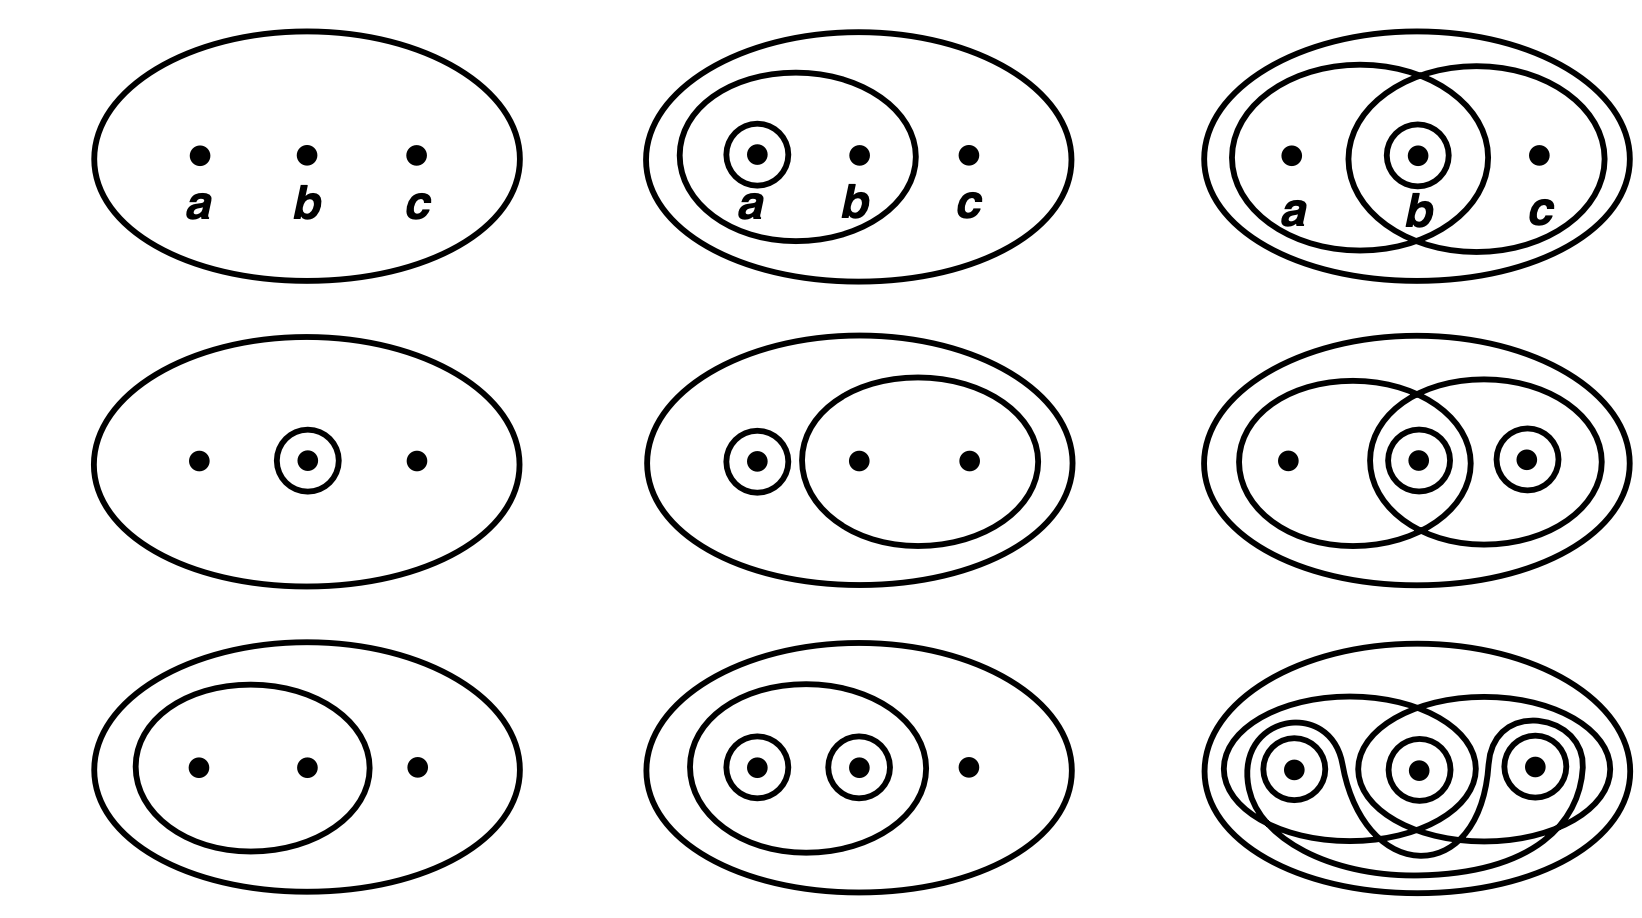
\includegraphics[scale=0.3]{img/top.png}
      \caption{} 
      \label{fig:top}
    \end{figure} 
    $\tau_{11}$ is the indiscrete topology so $\tau_{11} \subset \tau_{i, j}$ for all $i, j$, i.e. it is coarsest. $\tau_{33}$ is the discrete topology so $\tau_{i, j} \subset \tau_{3, 3}$ for all $i, j$, i.e. it is the finest. We list all other comparable topologies below. 
    \begin{enumerate}
      \item $\tau_{1, 2} \subset \tau_{3, 2}, \tau_{1, 3}, \tau_{2, 3}$. 
      \item $\tau_{3, 1} \subset \tau_{1, 2}, \tau_{3, 2}, \tau_{1, 3}, \tau_{2, 3}$. 
      \item $\tau_{1, 2} \subset \tau_{3, 2}$. 
      \item $\tau_{1, 3} \subset \tau_{2, 3}$. 
    \end{enumerate}
  \end{solution}

  \begin{exercise}[Munkres 13.3]
    Show that the collection $\mathcal{T}_c$ given in Example 4 of \S12 is a topology on the set $X$. Is the collection
    \begin{align*}
      \mathcal{T}_\infty = \{U \mid X - U \text{ is infinite or empty or all of } X\}
    \end{align*}
    a topology on $X$?
  \end{exercise}
  \begin{solution}[Munkres 13.3]
    We denote $\mathcal{T}_c$ as the set of all subsets $U \subset X$ such that $X \setminus U$ is countable is all of $X$. We show the 4 properties: 
    \begin{enumerate}
      \item $U = \emptyset \implies X \setminus U = X$, which is by definition in $\mathcal{T}_c$. 
      \item $U = X \implies X \setminus U = \emptyset$, which has cardinality $0$. Therefore it is countable and is in $\mathcal{T}_c$. 

      \item Let $\{U_\alpha\}_{\alpha \in I} \in \mathcal{T}_c$ by a collection of open sets of $X$. Then 
      \begin{equation}
        X \setminus \bigcup_{\alpha \in I} U_{\alpha} = \bigcap_{\alpha \in I} (X \setminus U_\alpha)
      \end{equation}
      $X \setminus U_\alpha$ is countable for all $\alpha \in I$, so let us fix some $\alpha^\prime$. Then 
      \begin{equation}
        \bigcap_{\alpha \in I} (X \setminus U_\alpha) \subset U_{\alpha^\prime} \implies \bigg| \bigcap_{\alpha \in I} (X \setminus U_\alpha) \bigg| \leq \big| U_{\alpha^\prime} \big| 
      \end{equation}
      and so the intersection is also countable. 
      \item Let $\{U_i\}_{i=1}^n$ by a finite collection of open sets of $X$. Then 
      \begin{equation}
        X \setminus \bigcap_{i=1}^n U_i = \bigcup_{i=1}^n (X \setminus U_i)
      \end{equation}
      Since $U_i$ are open, $X \setminus U_i$ are countable, and since the finite union of countable sets are countable, the RHS is countable, which implies the LHS is countable and so $\cap_{i=1}^n U_i$ is open as well. 
    \end{enumerate}

    As for $\mathcal{T}_\infty$, it is not a topology. Let us take $X = \mathbb{R}$, and look at the sets $\mathbb{Z}_{\geq 0}, \mathbb{Z}_{\leq 0}$ consisting of all the non-negative and non-positive integers. They are both infinite, and so $\mathbb{R} \setminus \mathbb{Z}_{\geq 0}$ and $\mathbb{R} \setminus \mathbb{Z}_{\leq 0}$ are in $\mathcal{T}_\infty$. Consider their union. 
    \begin{equation}
      (\mathbb{R} \setminus \mathbb{Z}_{\geq 0}) \cup (\mathbb{R} \setminus \mathbb{Z}_{\leq 0}) = \mathbb{R} \setminus (\mathbb{Z}_{\geq 0} \cap \mathbb{Z}_{\leq 0}) = \mathbb{R} \setminus \{0\}
    \end{equation}
    But $\mathbb{R} \setminus (\mathbb{R} \setminus \{0\}) = \{0\}$, and so $\mathbb{R} \setminus \{0\}$ is not open. Therefore $\mathcal{T}_c$ doesn't satisfy the definition of a topology. 
  \end{solution}

  \begin{exercise}[Munkres 13.4]
    (a) If $\{\mathcal{T}_\alpha\}$ is a family of topologies on $X$, show that $\bigcap \mathcal{T}_\alpha$ is a topology on $X$. Is $\bigcup \mathcal{T}_\alpha$ a topology on $X$?
    
    (b) Let $\{\mathcal{T}_\alpha\}$ be a family of topologies on $X$. Show that there is a unique smallest topology on $X$ containing all the collections $\mathcal{T}_\alpha$, and a unique largest topology contained in all $\mathcal{T}_\alpha$.
    
    (c) If $X = \{a, b, c\}$, let
    \begin{align*}
      \mathcal{T}_1 = \{\emptyset, X, \{a\}, \{a, b\}\} \quad \text{and} \quad \mathcal{T}_2 = \{\emptyset, X, \{a\}, \{b, c\}\}.
    \end{align*}
    Find the smallest topology containing $\mathcal{T}_1$ and $\mathcal{T}_2$, and the largest topology contained in $\mathcal{T}_1$ and $\mathcal{T}_2$.
  \end{exercise}
  \begin{solution}
    
  \end{solution}

  \begin{exercise}[Munkres 13.5]
    Show that if $\mathcal{A}$ is a basis for a topology on $X$, then the topology generated by $\mathcal{A}$ equals the intersection of all topologies on $X$ that contain $\mathcal{A}$. Prove the same if $\mathcal{A}$ is a subbasis.
  \end{exercise}
  \begin{solution}
    
  \end{solution}

  \begin{exercise}[Munkres 17.1]
    Let $\mathcal{C}$ be a collection of subsets of the set $X$. Suppose that $\emptyset$ and $X$ are in $\mathcal{C}$, and that finite unions and arbitrary intersections of elements of $\mathcal{C}$ are in $\mathcal{C}$. Show that the collection
    \begin{align*}
      \mathcal{T} = \{X - C \mid C \in \mathcal{C}\}
    \end{align*}
    is a topology on $X$.
  \end{exercise}
  \begin{solution}
    
  \end{solution}

  \begin{exercise}[Munkres 17.2]
    Show that if $A$ is closed in $Y$ and $Y$ is closed in $X$, then $A$ is closed in $X$.
  \end{exercise}
  \begin{solution}
    
  \end{solution}

  \begin{exercise}[Munkres 17.3]
    Show that if $A$ is closed in $X$ and $B$ is closed in $Y$, then $A \times B$ is closed in $X \times Y$.
  \end{exercise}
  \begin{solution} 
    It suffices to prove that $(X \times Y) \setminus (A \times B)$ is open. 
    \begin{align}
      (X \times Y) \setminus (A \times B) & \coloneqq \{ (x, y) \in X \times Y \mid (x \not\in A) \lor (y \not\in B) \} \\
                                          & = \{(x, y) \in X \times Y \mid x \not\in A \} \cup \{(x, y) \in X \times Y \mid y \not\in B \} \\
                                          & = [(X \setminus A) \times Y] \cup [X \times (Y \setminus B)]
    \end{align}
    We know that since $A, B$ are closed, $X \setminus A, Y \setminus B$ are open. Therefore each the expressions under definition of the product topology are open and their union must also be open. 
  \end{solution}

  \begin{exercise}[Munkres 17.4]
    Show that if $U$ is open in $X$ and $A$ is closed in $X$, then $U - A$ is open in $X$, and $A - U$ is closed in $X$.
  \end{exercise}
  \begin{solution}
    We know that $U^c$ is closed and $A^c$ is open. Since $U \setminus A = U \cap A^c$, it is the finite intersection of two open sets and therefore is open. Since $A \setminus U = A \cap U^c$, is an intersection of two closed sets, it is closed. 
  \end{solution}

  \begin{exercise}[Munkres 17.5]
    Let $X$ be an ordered set in the order topology. Show that $\overline{(a, b)} \subset [a, b]$. Under what conditions does equality hold?
  \end{exercise}
  \begin{solution}
    
  \end{solution}

  \begin{exercise}[Munkres 17.6]
    Let $A$, $B$, and $A_\alpha$ denote subsets of a space $X$. Prove the following:
    \begin{enumerate}
      \item If $A \subset B$, then $\bar{A} \subset \bar{B}$.
      \item $\overline{A \cup B} = \bar{A} \cup \bar{B}$.
      \item $\bigcup \bar{A}_\alpha \supset \overline{\bigcup A_\alpha}$; give an example where equality fails.
    \end{enumerate}
  \end{exercise}
  \begin{solution}
    For the first part, let $x \in \overline{A}$. If $x \in A$, then $x \in B \subset \overline{B}$ and we are done. If $x \in A^\prime$, then by definition every punctured neighborhood $U_x^\circ$ has a nonempty intersection with $A$, i.e. $U_x^\circ \cap A \neq \emptyset$ for any $U_x$. Choose $y \in U_x^\circ \cap A$. Since $y \in A \subset B$, this means that $y \in U_x^\circ \cap B$, which proves that $A^\prime \subset B^\prime$. 

    For the second part, we show bidirectionally. 
    \begin{enumerate}
      \item $\overline{A} \cup \overline{B} \subset \overline{A \cup B}$. WLOG let $x \in \overline{A}$. If $x \in A$, then $x \in (A \cup B) \subset \overline{A \cup B}$. If $x \not\in A$, then $x \in A^\prime$. Therefore for every $U_x^\circ$, $U_x^\circ \cap A \neq \emptyset$. But this means 
      \begin{equation}
        \emptyset \neq (U_x^\circ \cap A) \cup (U_x^\circ \cap B) = U_x^\circ \cap (A \cup B) \implies x \in (A \cup B)^\prime \subset \overline{A \cup B}
      \end{equation}

      \item $\overline{A \cup B} \subset \overline{A} \cup \overline{B}$. Let $x \in \overline{A \cup B}$. If $x \in A \cup B$, then it must be the case that either $x \in A \subset (A \cup A^\prime) = \overline{A}$ or $x \in B \subset (B \cup B^\prime) = \overline{B}$, which means $x \in \overline{A} \cup \overline{B}$. If not, then $x \in (A \cup B)^\prime$, and therefore for all $U_x^\circ$, 
      \begin{equation}
        U_x^\circ \cap (A \cup B) \neq \emptyset \implies (U_x^\circ \cap A) \cup (U_x^\circ \cap B) \neq \emptyset
      \end{equation}
      Now assume $x$ is not a limit point of $A$ and not a limit point of $B$. Then there exists open neighborhoods $U^1_x$ and $U^2_x$ such that $(U_x^1 \setminus \{x\}) \cap A = \emptyset$ and $(U_x^2 \setminus \{x\}) \cap B = \emptyset$. But since $V_x = U_x^1 \cap U_x^2$ is also open, $V_x^\circ \coloneqq V_x \setminus \{x\}$ is also a existing punctured neighborhood that has a trivial intersection with $A$ and that with $B$. 
      \begin{align}
        V_x^\circ \cap A & = \big( [U_x^1 \cap U_x^2] \setminus \{x\} \big) \cap A \\
                         & = \big( [U_x^1 \setminus \{x\}] \cap [U_x^2 \setminus \{x\}] \big) \cap A \\
                         & = ([U_x^1 \setminus \{x\}] \cap A) \cap ([U_x^2 \setminus \{x\}] \cap A) \\ 
                         & = \emptyset \cap ([U_x^2 \setminus \{x\}] \cap A) = \emptyset
      \end{align}
      and the analogous argument follows for $B$. This means that $V_x^\circ \cap (A \cup B) = (V_x^\circ \cap A) \cup (V_x^\circ \cap B) = \emptyset$, contradicting the fact that $x \in (A \cup B)^\prime$. Therefore $x$ must be a limit point of at least one of $A$ or $B$. 
    \end{enumerate}

    For the third, assume that $x \in \bigcup \overline{A_\alpha}$. Then there exists an $\alpha^\ast$ s.t. $x \in \overline{A_{\alpha^\ast}}$. We know from (1) that 
    \begin{equation}
      A_{\alpha^\ast} \subset \bigcup_{\alpha} A_\alpha \implies \overline{A_{\alpha^\ast}} \subset \overline{\bigcup_{\alpha} A_\alpha} 
    \end{equation}
    and so $x \in \overline{\bigcup A_\alpha}$. A counterexample follows from the idea that we've depended on $V_x$ being a \textit{finite} intersection open open sets from before. Consider the set of singletons $A_\alpha = \alpha$ for $\alpha \in (0, 1)$. Then
    \begin{equation}
      \overline{\bigcup_{\alpha \in (0, 1)} A_\alpha} = \overline{(0, 1)} = [0, 1] \neq (0, 1) = \bigcup_{\alpha \in (0, 1)} \{\alpha\} = \bigcup_{\alpha \in (0, 1)} \overline{\{\alpha\}} =  \bigcup_{\alpha \in (0, 1)} \overline{A_\alpha} 
    \end{equation}
  \end{solution}

  \begin{exercise}[Munkres 17.7]
    Criticize the following ``proof'' that $\bigcup \bar{A}_\alpha \subset \overline{\bigcup A_\alpha}$: if $\{A_\alpha\}$ is a collection of sets in $X$ and if $x \in \bigcup \bar{A}_\alpha$, then every neighborhood $U$ of $x$ intersects $\bigcup A_\alpha$. Thus $U$ must intersect some $A_\alpha$, so that $x$ must belong to the closure of some $A_\alpha$. Therefore, $x \in \bigcup \bar{A}_\alpha$.
  \end{exercise}
  \begin{solution}
    
  \end{solution}

  \begin{exercise}[Munkres 17.8]
    Let $A$, $B$, and $A_\alpha$ denote subsets of a space $X$. Determine whether the following equations hold; if an equality fails, determine whether one of the inclusions $\supset$ or $\subset$ holds.
    \begin{enumerate}
      \item $\bar{A} \cap \bar{B} = \overline{A \cap B}$.
      \item $\bigcap \bar{A}_\alpha = \overline{\bigcap A_\alpha}$.
      \item $\bar{A} - \bar{B} = \overline{A - B}$.
    \end{enumerate}
  \end{exercise}
  \begin{solution}
    
  \end{solution}

  \begin{exercise}[Munkres 17.9]
    Let $A \subset X$ and $B \subset Y$. Show that in the space $X \times Y$,
    \begin{align*}
      \overline{A \times B} = \bar{A} \times \bar{B}.
    \end{align*}
  \end{exercise}
  \begin{solution}
    
  \end{solution}

  \begin{exercise}[Munkres 17.10]
    Show that every order topology is Hausdorff.
  \end{exercise}
  \begin{solution}
    
  \end{solution}

  \begin{exercise}[Munkres 17.11]
    Show that the product of two Hausdorff spaces is Hausdorff.
  \end{exercise}
  \begin{solution}
    Given two Hausdorff spaces $(X, \T_X), (Y, \T_Y)$, we will denote their product space as $(X \times Y, \T_{X \times Y})$. Let us have two points $(x_1, y_1), (x_2, y_2) \in X \times Y$. Then $x_1, x_2 \in X$, and since $X$ is Hausdorff there exists $U_1, U_2 \in \T_X$ containing $x_1, x_2$ respectively such that $U_1 \cap U_2 = \emptyset$. By similar logic we have $V_1, V_2 \in \T_Y$ containing $y_1, y_2$. Then, $(x_1, y_1) \in U_1 \times V_1$ open and $(x_2, y_2) \in U_2 \times V_2$ open, and we claim that $(U_1 \times V_1) \cap (U_2 \times V_2) = \emptyset$. If not, then there exists a $(x^\prime, y^\prime)$ contained in both sets, but this implies that $x^\prime \in U_1 \cap U_2$ contradicting the fact that $X$ is Hausdorff. Therefore $(U_1 \times V_1)$ and $(U_2 \times V_2)$ are disjoint and we have shown such a construction. 
  \end{solution}

  \begin{exercise}[Munkres 17.12]
    Show that a subspace of a Hausdorff space is Hausdorff.
  \end{exercise}
  \begin{solution}
    Let $(X, \T_X)$ be Hausdorff and $(Y, \T_Y)$ be a subspace of $X$ with the subspace topology of $X$. Choose two points $y_1, y_2 \in Y$. Then as elements of $X$ there exists disjoint $U_1, U_2 \in \T_X$ containing $y_1, y_2$ respectively. Therefore, letting $V_1 = U_1 \cap Y$ and $V_2 = U_2 \cap Y$ be open sets in $\T_Y$, we have 
    \begin{equation}
      V_1 \cap V_2 = (U_1 \cap Y) \cap (U_2 \cap Y) = (U_1 \cap U_2) \cap Y = \emptyset 
    \end{equation}
    Therefore we have constructed two open sets containing $y_1, y_2$ that are disjoint, and so $(Y, \T_Y)$ is Hausdorff. 
  \end{solution}

  \begin{exercise}[Munkres 17.13]
    Show that $X$ is Hausdorff if and only if the diagonal $\Delta = \{x \times x \mid x \in X\}$ is closed in $X \times X$.
  \end{exercise}
  \begin{solution}
    We prove bidirectionally. 
    \begin{enumerate}
      \item $(\rightarrow)$. $X$ is Hausdorff implies $X \times X$ is Hausdorff. We wish to show that a $(X \times X) \setminus \Delta$ is open. So pick a point $x \not\in \Delta$, which must be of form $(x_1, x_2)$ for $x_1 \neq x_2$. Since $X$ is Hausdorff, there exists disjoint open sets $U_1 \ni x_1, U_2 \ni x_2$. Therefore, consider the open set $U_1 \times U_2$, which must consist of points $(z_1, z_2)$ where $z_1 \in U_1, z_2 \in U_2$. Therefore $z_1 \neq z_2$, and so $(U_1 \times U_2) \cap \Delta = \emptyset$, and so it is contained within $(X \times X) \setminus \Delta$, i.e. is open. 

      \item $(\leftarrow)$ Assume that $\Delta$ is closed in $X \times X$, i.e. $(X \times X) \setminus \Delta$ is open. We look at the point $(x_1, x_2) \in (X \times X) \setminus \Delta$, which implies $x_1 \neq x_2$. By openness of $(X \times X) \setminus \Delta$, there exists an open set $U_{(x_1, x_2)} \ni (x_1, x_2)$ in $(X \times X) \setminus \Delta$, which we can write as a basis element $U_1 \times U_2$ for open $U_1 \ni x_1, U_2 \ni x_2$ in $X$.\footnote{Since the basis of the product topology is already defined and choosing $(x_1, x_2)$ by definition of a basis such a basis element must exist containing $(x_1, x_2)$.} Note that since $(U_1 \times U_2) \cap \Delta = \emptyset$, $U_1 \times U_2$ cannot contain a point of the form $(x, x)$, implying that both $U_1$ and $U_2$ cannot contain the same element $x$, which implies that $U_1, U_2$ are disjoint. Therefore $X$ is Hausdorff. 
    \end{enumerate} 

  \end{solution}

  \begin{exercise}[Munkres 17.14]
    In the finite complement topology on $\mathbb{R}$, to what point or points does the sequence $x_n = 1/n$ converge?
  \end{exercise}
  \begin{solution}
    It converges to every point $x \in \mathbb{R}$. Take any $x \in \mathbb{R}$, then we wish to show that for every open neighborhood $U_x$ there exists an $N \in \mathbb{N}$ s.t. $x_n \in U_x$ for every $n > N$. Every $U_x$ must be all of $\mathbb{R}$ minus a finite set $S$. The intersection $S \cap \{x_n\}$ must be finite so there is a maximum index $N$ such that $x_N \not\in U_x$. Therefore, for all $n > N$, $x_n \not\in S \implies x_n \in U_x$. 
  \end{solution}

  \begin{exercise}[Munkres 17.15]
    Show the $T_1$ axiom is equivalent to the condition that for each pair of points of $X$, each has a neighborhood not containing the other.
  \end{exercise}
  \begin{solution}
    
  \end{solution}

  \begin{exercise}[Munkres 17.16]
    Consider the five topologies on $\mathbb{R}$ given in Exercise 7 of \S13.
    \begin{enumerate}
      \item Determine the closure of the set $K = \{1/n \mid n \in \mathbb{Z}_+\}$ under each of these topologies.
      \item Which of these topologies satisfy the Hausdorff axiom? the $T_1$ axiom?
    \end{enumerate}
  \end{exercise}
  \begin{solution}
    
  \end{solution}

  \begin{exercise}[Munkres 17.17]
    Consider the lower limit topology on $\mathbb{R}$ and the topology given by the basis $\mathcal{C}$ of Exercise 8 of \S13. Determine the closures of the intervals $A = (0, \sqrt{2})$ and $B = (\sqrt{2}, 3)$ in these two topologies.
  \end{exercise}
  \begin{solution}
    
  \end{solution}

  \begin{exercise}[Munkres 17.18]
    Determine the closures of the following subsets of the ordered square:
    \begin{align*}
      A &= \{(1/n) \times 0 \mid n \in \mathbb{Z}_+\}, \\
      B &= \{(1 - 1/n) \times \frac{1}{2} \mid n \in \mathbb{Z}_+\}, \\
      C &= \{x \times 0 \mid 0 < x < 1\}, \\
      D &= \{x \times \frac{1}{2} \mid 0 < x < 1\}, \\
      E &= \{\frac{1}{2} \times y \mid 0 < y < 1\}.
    \end{align*}
  \end{exercise}
  \begin{solution}
    
  \end{solution}

  \begin{exercise}[Munkres 17.19]
    If $A \subset X$, we define the \textit{boundary} of $A$ by the equation
    \begin{align*}
      \text{Bd } A = \bar{A} \cap \overline{(X - A)}.
    \end{align*}
    
    \begin{enumerate}
      \item Show that $\text{Int } A$ and $\text{Bd } A$ are disjoint, and $\bar{A} = \text{Int } A \cup \text{Bd } A$.
      \item Show that $\text{Bd } A = \emptyset \Leftrightarrow A$ is both open and closed.
      \item Show that $U$ is open $\Leftrightarrow \text{Bd } U = \bar{U} - U$.
      \item If $U$ is open, is it true that $U = \text{Int}(\bar{U})$? Justify your answer.
    \end{enumerate}
  \end{exercise}
  \begin{solution}
    
  \end{solution}

  \begin{exercise}[Munkres 17.20]
    Find the boundary and the interior of each of the following subsets of $\mathbb{R}^2$:
    \begin{enumerate}
      \item $A = \{x \times y \mid y = 0\}$
      \item $B = \{x \times y \mid x > 0 \text{ and } y \neq 0\}$
      \item $C = A \cup B$
      \item $D = \{x \times y \mid x \text{ is rational}\}$
      \item $E = \{x \times y \mid 0 < x^2 - y^2 \leq 1\}$
      \item $F = \{x \times y \mid x \neq 0 \text{ and } y \leq 1/x\}$
    \end{enumerate}
  \end{exercise}
  \begin{solution}
    
  \end{solution}

  \begin{exercise}[Munkres 17.21]
    (Kuratowski) Consider the collection of all subsets $A$ of the topological space $X$. The operations of closure $A \to \bar{A}$ and complementation $A \to X - A$ are functions from this collection to itself.
    \begin{enumerate}
      \item Show that starting with a given set $A$, one can form no more than 14 distinct sets by applying these two operations successively.
      \item Find a subset $A$ of $\mathbb{R}$ (in its usual topology) for which the maximum of 14 is obtained.
    \end{enumerate}
  \end{exercise}
  \begin{solution}
    
  \end{solution}

\subsection{Common Topologies}

  \begin{exercise}[Munkres 13.6]
    Show that the topologies of $\mathbb{R}_\ell$ and $\mathbb{R}_K$ are not comparable.
  \end{exercise}
  \begin{solution}[Munkres 13.6]
    It suffices to show 2 things. Note that $K \coloneqq \{ 1/n \}_{n \in \mathbb{N}}$. 
    \begin{enumerate}
      \item \textit{$\mathcal{T}_\ell$ is not finer than $\mathcal{T}_K$}. Let $U = [-1, 1)$. Let $U = [0, 1) \in \mathscr{B}_\ell$ and $0 \in U$. We would like to show that there is no basis element of $\mathscr{B}_k$ that both contains $0$ and is contained in $U$. Assume that there is. It can be of form $(a, b)$ or $(a, b) \setminus K$. Assume the former. Then $0 \in (a, b) \implies a < 0$. Therefore $-a/2 \in (a, b)$, but $-a/2 \not\in [0, 1)$, so $(a, b) \not\subset U$. Therefore it must be of form $(a, b) \setminus K$. However, $K \cap \{0\} = \emptyset$, so $0 \in (a, b) \setminus K \implies 0 \in (a, b)$. But by the same logic as the first case, $(a, b) \setminus K \not\subset U$ since it must contain a negative number. Therefore our assumption is false, and $\mathcal{T}_{\ell}$ is not finer than $\mathcal{T}_K$. 
      \item \textit{$\mathcal{T}_K$ is not finer than $\mathcal{T}_\ell$}. Let $U = (-1, 1) \setminus K \in \mathscr{B}_K$ and $0 \in U$. Assume that there is a basis element $[a, b) \in \mathscr{B}_\ell$ such that $0 \in [a, b) \subset U$. $0 \in [a, b) \implies 0 < b$, but since $\mathbb{R}$ is Archimedean, there exists a $N \in \mathbb{N}$ s.t. $0 < 1/N < b$, and therefore $1/N \not\in U$. This contradicts the fact that $[a, b) \subset U$, and so no such $[a, b)$ exists. 
    \end{enumerate}
    Therefore by Munkres Lemma 13.3, neither is finer than the other, which by definition means they are incomparable. 
  \end{solution}


  \begin{exercise}[Munkres 13.7]
    Consider the following topologies on $\mathbb{R}$:
    \begin{align*}
      \mathcal{T}_1 &= \text{the standard topology}, \\
      \mathcal{T}_2 &= \text{the topology of } \mathbb{R}_K, \\
      \mathcal{T}_3 &= \text{the finite complement topology}, \\
      \mathcal{T}_4 &= \text{the upper limit topology, having all sets } (a, b] \text{ as basis}, \\
      \mathcal{T}_5 &= \text{the topology having all sets } (-\infty, a) = \{x \mid x < a\} \text{ as basis}.
    \end{align*}
    Determine, for each of these topologies, which of the others it contains.
  \end{exercise}
  \begin{solution}[Munkres 13.7]
    We claim 
    \begin{equation} 
      \T_3, \T_5 \subset \T_1 \subset \T_2, \T_4, \; \T_3 \not\sim \T_5, \; \T_2 \not\sim \T_4
    \end{equation} 
    where $\not\sim$ means that they are not comparable, and $\subset$ means proper subset (strictly finer). We show the following. 
    \begin{enumerate}
      \item $\T_3 \subset \T_1$. Let $x \in U_3 \in \T_3$. Then $\mathbb{R} \setminus U_3$ is finite. Therefore the following is defined. 
      \begin{equation}
        r = \min_{y \in (\mathbb{R} \setminus U_3)} |x - y| 
      \end{equation} 
      Therefore, construct the open ball $B(x, r) = (x - r, x + r)$. Since $y \in B(x, r) \implies |y - x| < d$, and every point $z \not\in U_3$ must satisfy $|z - x| \geq d$, we proved that $B(x, r) \subset U_3$. By definition this means that $U_3 \subset \T_1$. To show strictness, take the open ball $(0, 1) \in \mathscr{T}_1$. $\mathbb{R} \setminus (0, 1)$ is infinite, so $\mathscr{T}_1 \not\subset \T_3$.  

      \item $\T_5 \subset \T_1$. Given $x \in \mathbb{R}$, let us choose a $\T_5$-open neighborhood $(-\infty, a)$ containing $x$. Then, we construct the $\T_1$-open neighborhood of $x$ as $(x - 1, a) \subset (-\infty, a)$, and we are done. To show strictness, take the basis element $(0, 1) \in \mathscr{B}_1$ and set $x = 0.5$. Then every basis element of $\mathscr{B}_5$ containing $x$ is of form $(-\infty, a), a > 0.5$ and so contains $-1$. Therefore it cannot be a subset of $(0, 1)$ and so the topologies are not equal. 

      \item $\T_5 \not\sim \T_3$. Consider $U_5 = (-\infty, 0) \in \mathscr{T}_5$. Its complement $[0, -\infty)$ is infinite so $U_5 \not\in \mathscr{T}_3$. Consider $U_3 = (-\infty, 0) \cup (0, +\infty) \in \T_3$. If $U_3$ is open in $\T_5$, then it must be a union of the basis elements of form $(-\infty, a)$. Since $1 \in U_3$, at least one of the basis elements $B$ must have $a > 1$, but this means $0 \in B \implies 0 \in U_3$. This cannot happen and so $U_3$ is not open in $\T_5$. 

      \item $\T_1 \subset \T_2$ is proven in Munkres Lemma 13.4.  

      \item $\T_1 \subset \T_4$. Let $x \in \mathbb{R}$ and choose a basis element $(a, b) \in \mathscr{B}_1$ containing $x$. Then we choose the basis element $(a, x] \in \mathscr{B}_4$ which also contains $x$, and $a < x < b \implies (a, x] \subset (a, b)$. We are done. To show strictness, let us choose $x \in \mathbb{R}$ and choose basis element $(a, x]$. Then we claim there is no $\T_1$-open neighborhood of $x$ contained in $(a, x]$. Assume there was, of form $(c, d)$. Then $x < d$, and by density of rationals there exists a $q$ such that $x < q < d$. Then $q \in (c, d)$ but $q \not\in (a, x]$, and $(c, d) \not\subset (a, x]$. By contradiction, there exists no subset, and $\T_1 \not\supset \T_4$. 

      \item $\T_2 \not\sim \T_4$. Consider $U_2 = (0, 1.1) \setminus K \in \T_2$. Note that $\frac{2}{19}, \frac{21}{20} \in U_2$. Now assume that there is some basis element $(a, b]$ of $\T_4$ that is contained in $U_2$. It must be the case that $a < 2/19$ and $b \geq 21/20$, but this means that $1/2 \in (a, b]$, which is not in $U_2$. Therefore, $\T_4$ is not finer than $\T_2$. 

      For the other direction, consider $x = 2$ and $U_4 = (1, 2] \in \mathscr{B}_2$. We claim that there is no basis element of $\T_4$ that contains $x$ and is contained in $U_4$. From point 5 above, the basis element cannot be of form $(a, b)$. So it must be of form $(a, b) \setminus K$. Assume that there was such a set. Then $(a, b) \setminus K \subset (1, 2]$, but this means that $b > 2$. Therefore by the same reasoning above, there must exist some $q$ s.t. $2 < q < b$, and so $q \in (a, b) \setminus K$ but $q \not\in (1, 2]$. Therefore $\T_2$ is not finer than $\T_4$. 
    \end{enumerate}
  \end{solution}

  \begin{exercise}[Munkres 13.8]
    (a) Apply Lemma 13.2 to show that the countable collection
    \begin{align*}
      \mathcal{B} = \{(a, b) \mid a < b, a \text{ and } b \text{ rational}\}
    \end{align*}
    is a basis that generates the standard topology on $\mathbb{R}$.
    
    (b) Show that the collection
    \begin{align*}
      \mathcal{C} = \{[a, b) \mid a < b, a \text{ and } b \text{ rational}\}
    \end{align*}
    is a basis that generates a topology different from the lower limit topology on $\mathbb{R}$.
  \end{exercise}
  \begin{solution}[Munkres 13.8]
    Listed. 
    \begin{enumerate}
      \item For any open set $U \subset \mathbb{R}$ and $x \in U$, by definition there exists a $r > 0$ s.t. $B(x, r) = (x - r, x + r) \subset U$. But by the density of the rationals in $\mathbb{R}$, there exists an $a, b \in \mathbb{Q}$ s.t. 
      \begin{equation}
        x - r < a < x < b < x + r \implies x \in (a, b) \subset (x - r, x + r) \subset U
      \end{equation}
      Since we can always find such an element $(a, b) \in \mathcal{B}$ satisfying $x \in (a, b) \subset U$, $\mathcal{B}$ is a basis.  

    \item Call the topology generated by $\mathscr{C}$ to be $\mathscr{T}$, and let the lower limit topology be $\mathscr{T}^\prime$ generated by its corresponding basis, denoted $\mathscr{B}$. Assume that $\mathscr{T} = \mathscr{T}^\prime$. Then, $\mathscr{T}^\prime \subset \mathscr{T}$, and by Lemma 13.2, it must be the case that for each $x \in X$ and basis element $B \in \mathscr{B}$, we can find a $C \in \mathscr{C}$ s.t. $x \in C \subset B$. Consider $x = \sqrt{2}$ and $B = [\sqrt{2}, 2)$. We attempt to find an interval $[a, b)$ with $a, b \in \mathbb{Q}$ such that $\sqrt{2} \in [a, b)\subset[\sqrt{2}, 2)$. Clearly $a \neq \sqrt{2}$ since $a$ is rational. If $a > \sqrt{2}$, then $x \not\in [a, b)$. If $a < \sqrt{2}$, then by density of rationals in $\mathbb{R}$, there exists a $q \in \mathbb{Q}$ satisfying $a < q < \sqrt{2}$. Therefore, there exists a $q \in \mathbb{R}$ s.t. $q \in [a, b)$ but $q \not\in [\sqrt{2}, 2)$, implying that $[a, b) \not\subset [\sqrt{2}, 2)$. Therefore such an interval cannot exist $\implies \mathscr{T}^\prime \not\subset \mathscr{T} \implies \mathscr{T}^\prime \neq \mathscr{T}$.
    \end{enumerate}
  \end{solution}

  \begin{exercise}[Munkres 20.1]
    (a) In $\mathbb{R}^n$, define
    \begin{align*}
      d'(\mathbf{x}, \mathbf{y}) = |x_1 - y_1| + \cdots + |x_n - y_n|.
    \end{align*}
    Show that $d'$ is a metric that induces the usual topology of $\mathbb{R}^n$. Sketch the basis elements under $d'$ when $n = 2$.
    
    (b) More generally, given $p \geq 1$, define
    \begin{align*}
      d'(\mathbf{x}, \mathbf{y}) = \left[\sum_{i=1}^{n} |x_i - y_i|^p\right]^{1/p}
    \end{align*}
    for $\mathbf{x}, \mathbf{y} \in \mathbb{R}^n$. Assume that $d'$ is a metric. Show that it induces the usual topology on $\mathbb{R}^n$.
  \end{exercise}
  \begin{solution}[Munkres 20.1.a] 
    Let $\mathscr{B}_1, \mathscr{B}_2$ be the basis of open balls with respect to the $d^\prime = d_1$ and $d_2$ metrics on $\mathbb{R}^n$, with their generated topologies being $\mathscr{T}_1, \mathscr{T}_2$. We show that 
    \begin{equation}
      d_2 (x, y) \leq d_1 (x, y) \leq \sqrt{n} d_2 (x, y)
    \end{equation} 
    Since all expressions are nonnegative, it suffices to show that 
    \begin{equation}
      (d_2 (x, y))^2 \leq (d_1 (x, y))^2 \leq n (d_2 (x, y))^2
    \end{equation} 
    \begin{enumerate}
      \item $d_2 (x, y))^2 \leq (d_1 (x, y))^2$. We see that by expanding and seeing that the product of absolute values is always nonnegative, 
      \begin{align}
        (d_1 (x, y))^2 & = \bigg( \sum_i |x_i - y_i| \bigg)^2 \\
                       & = \sum_i (x_i - y_i)^2 + \sum_{i \neq j} |x_i - y_i| |x_j - y_j| \\ 
                       & \geq \sum_i (x_i - y_i)^2 \\
                       & = (d_2 (x, y))^2
      \end{align}

      \item For the second part, we use the Schwartz inequality. 
      \begin{align}
        d_1 (x, y) & = \sum_i |x_i - y_i| \\ 
                   & = \sum_i |x_i - y_i| \cdot 1 \\
                   & \leq \sqrt{\sum_i (x_i - y_i)^2} \cdot \sqrt{\sum_i 1} \\
                   & = d_2 (x, y) \cdot \sqrt{n}
      \end{align}
    \end{enumerate}
    Now we show that $\T_1 = \T_2$. 
    \begin{enumerate} 
      \item $\T_2 \subset \T_1$. Given an $\T_2$-open neighborhood $U$ and $x \in U$, by definition there exists a $r > 0$ s.t. $x \in B_2 (x, r) \subset U$. We claim that there exists a $r^\prime > 0$ such that $B_1 (x, r^\prime) \subset U$, making this also a $\T_1$-open neighborhood. Set $r^\prime = r$. Then 
      \begin{align}
        y \in B_1 (x, r) & \implies d_1 (x, y) < r \\
                         & \implies d_2 (x, y) \leq d_1 (x, y) < r \\
                         & \implies d_2 (x, y) < r \\
                         & \implies y \in B_2 (x, r)
      \end{align}
      and so $x \in B_1 (x, r) \subset B_2 (x, r) \subset U$. 

      \item $\T_1 \subset \T_2$. Given an $\T_1$-open neighborhood $U$ and $x \in U$, by definition there exists a $r > 0$ s.t. $x \in B_1 (x, r) \subset U$. We claim that there exists a $r^\prime > 0$ such that $B_2 (x, r^\prime) \subset U$, making this also a $\T_2$-open neighborhood. Set $r^\prime = r n^{-1/2}$. Then 
      \begin{align}
        y \in B_2 (x, r n^{-1/2}) & \implies d_2 (x, y) < r n^{-1/2} \\
                                  & \implies n^{1/2} d_2 (x, y) < r \\ 
                                  & \implies d_1 (x, y) < r \\
                                  & \implies y \in B_1 (x, r) 
      \end{align}
      and so $x \in B_2 (x, r) \subset B_1 (x, r) \subset U$. 
    \end{enumerate}  
  \end{solution}

  \begin{solution}[Munkres 20.1.b]
    Let the metric be denoted $d_p (x, y)$. Let $q$ be the Holder conjugate of $p$, i.e. the unique $q \in \mathbb{R}$ s.t. $(1/p) + (1/q) = 1$. If $p = 1$, then we have proved the equivalence in (a). If $p > 1$, then by the ordered field properties of $\mathbb{R}$, $0 < 1/p < 1 \implies 0 < 1/q < 1 \implies q > 1$. Given that we can always define $q$, we show two things. 
    \begin{enumerate}
      \item $d_1 (x, y) \leq n^{1/q} d_p (x, y) \iff n^q d_1 (x, y) \leq d_p (x, y)$. 
      \begin{align}
        d_1 (x, y) & = \sum_i |x_i - y_i| \\ 
                   & = \sum_i |x_i - y_i| \cdot 1 \\
                   & \leq \bigg( \sum_i |x_i - y_i|^p \bigg)^{1/p} \cdot \bigg(\sum_i 1^q \bigg)^{1/q} \\
                   & = d_p (x, y) \cdot n^{1/q}
      \end{align} 

      \item $d_p (x, y) \leq n^{1/p} d_\infty (x, y) \iff n^p d_p (x, y) \leq d_\infty (x, y)$. Since both expressions are nonnegative (since we assumed that it's a metric), it suffices to prove that $(d_p (x, y))^p \leq (d_\infty (x, y))^{p}$. 
      \begin{align}
        (d_p(x, y))^p & = \sum_i |x_i - y_i|^p \\
                      & \leq \sum_i \big( \max_i \{ |x_i - y_i| \} \big)^p \\
                      & = n \cdot \big( \max_i \{ |x_i - y_i| \} \big)^p \\ 
                      & = n \cdot (d_\infty (x, y))^p \\
        d_p(x, y)     & = n^{1/p} \cdot d_\infty (x, y)
      \end{align}
    \end{enumerate} 
    Now we prove the following. Since $p = 1$ is proved in (a), we assume $p > 1$, and $q > 1$ is always defined. For notation, let $\T_p$ denote the topology generated by the basis of open balls $B_p (x, r)$ with respect to the $d_p$ metric. 

    \begin{enumerate} 
      \item $\T_1 \subset \T_p$. Let $U$ be open in $\T_1$ and $x \in U$. Then by definition there exists a $r > 0$ s.t. $x \in B_1 (x, r) \subset U$. We claim that there exists a $r^\prime$ s.t. $B_p (x, r^\prime) \subset U$, making this also a $\T_p$-open neighborhood. Set $r^\prime = r n^q$. 
      \begin{align}
        y \in B_p (x, r^\prime) & \implies d_p (x, y) < r n^q \\
                                & \implies n^q \cdot d_1 (x, y) \leq d_p (x, y) < r n^q \\
                                & \implies d_1 (x, y) < r \\
                                & \implies y \in B_1 (x, y)
      \end{align}
      Therefore $x \in B_p (x, r^\prime) \subset B_1 (x, y) \subset U$. 

      \item $\T_p \subset \T_\infty$. Let $U$ be open in $\T_p$ and $x \in U$. Then by definition there exists a $r > 0$ s.t. $x \in B_p (x, r) \subset U$. We claim that there exists $r^\prime$ s.t. $B_\infty (x, r^\prime) \subset U$, making this also a $\T_\infty$-open neighborhood. Set $r^\prime = r n^p$. 
      \begin{align}
        y \in B_\infty (x, r^\prime) & \implies d_\infty (x, y) < r n^q \\
                                     & \implies n^q d_p (x, y) \leq d_\infty (x, y) < r n^q  \\
                                     & \implies d_p (x, y) < r \\
                                     & \implies y \in B_p (x, r)
      \end{align}
      Therefore, $x \in B_\infty (x, r n^q) \subset B_p (x, r) \subset U$. 
    \end{enumerate} 

    From (a) and the previous homework, we know that $\T_1 = \T_\infty = \T_2$, denote this $\T$. Therefore, we have proved that $\T \subset \T_p$ and $\T_p \subset \T$, which means $\T = \T_p$. 
  \end{solution}

\subsection{Continuity}

  \begin{exercise}[Munkres 18.1]
    Prove that for functions $f : \mathbb{R} \to \mathbb{R}$, the $\epsilon$-$\delta$ definition of continuity implies the open set definition.
  \end{exercise}

  \begin{exercise}[Munkres 18.2]
    Suppose that $f : X \to Y$ is continuous. If $x$ is a limit point of the subset $A$ of $X$, is it necessarily true that $f(x)$ is a limit point of $f(A)$?
  \end{exercise}
  \begin{solution}
    No. Consider $X = Y = \mathbb{R}$ with the Euclidean topology and let $f(x) = 0$. Consider $A = (-1, 1) \implies f(A) = \{0\}$. $1$ is a limit point of $A$ but $f(1) = 0$ is not a limit point of $\{0\}$ since it's an isolated point, i.e. for any punctured open neighborhood $U_0^\circ = U_0 \setminus \{0\}$, 
    \begin{equation}
      U_0^\circ \cap f(A) = (U_0 \setminus \{0\}) \cap \{0\} = \emptyset
    \end{equation}
  \end{solution}

  \begin{exercise}[Munkres 18.3]
    Let $X$ and $X'$ denote a single set in the two topologies $\mathcal{T}$ and $\mathcal{T}'$, respectively. Let $i : X' \to X$ be the identity function.
    \begin{enumerate}
      \item Show that $i$ is continuous $\Leftrightarrow \mathcal{T}'$ is finer than $\mathcal{T}$.
      \item Show that $i$ is a homeomorphism $\Leftrightarrow \mathcal{T}' = \mathcal{T}$.
    \end{enumerate}
  \end{exercise}

  \begin{exercise}[Munkres 18.4]
    Given $x_0 \in X$ and $y_0 \in Y$, show that the maps $f : X \to X \times Y$ and $g : Y \to X \times Y$ defined by
    \begin{align*}
      f(x) = x \times y_0 \quad \text{and} \quad g(y) = x_0 \times y
    \end{align*}
    are imbeddings.
  \end{exercise}

  \begin{exercise}[Munkres 18.5]
    Show that the subspace $(a, b)$ of $\mathbb{R}$ is homeomorphic with $(0, 1)$ and the subspace $[a, b]$ of $\mathbb{R}$ is homeomorphic with $[0, 1]$.
  \end{exercise}

  \begin{exercise}[Munkres 18.6]
    Find a function $f : \mathbb{R} \to \mathbb{R}$ that is continuous at precisely one point.
  \end{exercise}

  \begin{exercise}[Munkres 18.7]
    \begin{enumerate}
      \item Suppose that $f : \mathbb{R} \to \mathbb{R}$ is ``continuous from the right,'' that is,
      \begin{align*}
        \lim_{x \to a^+} f(x) = f(a),
      \end{align*}
      for each $a \in \mathbb{R}$. Show that $f$ is continuous when considered as a function from $\mathbb{R}_\ell$ to $\mathbb{R}$.
      \item Can you conjecture what functions $f : \mathbb{R} \to \mathbb{R}$ are continuous when considered as maps from $\mathbb{R}$ to $\mathbb{R}_\ell$? As maps from $\mathbb{R}_\ell$ to $\mathbb{R}_\ell$? We shall return to this question in Chapter 3.
    \end{enumerate}
  \end{exercise}
  \begin{solution}
    This definition of continuity at a point in analysis means that for all $\epsilon > 0$ there exists a $\delta > 0$ s.t. $x \in [a, a + \delta) \implies |f(x) - f(a)| < \epsilon$. Assuming this definition holds, let $U_{f(a)} \in \T$ be an open neighborhood of $f(a)$ (w.r.t. Euclidean topology). We wish to show that the preimage is open in $\T_\ell$. 

    By definition of open sets in $\mathbb{R}$, there exists an open ball $(f(a) - \epsilon, f(a) + \epsilon) \subset U_{f(a)}$, and from our analytical definition of continuity there exists a $\delta > 0$ s.t. $f([a, a + \delta)) \subset (f(a) - \epsilon, f(a) + \epsilon)$. Therefore taking the preimage we have 
    \begin{equation}
      [a, a+\delta) \subset f^{-1} \big( (f(a) - \epsilon, f(a) + \epsilon ) \big) \subset f^{-1} \big( U_{f(a)} \big)
    \end{equation}
    Since we can construct an open ball (in $\T_\ell$) $[a, a + \delta) \subset f^{-1} (U_{f(a)})$, by definition $f^{-1} (U_{f(a)})$ is open in $\mathbb{R}_\ell$, making $f$ continuous at $a$. Since this holds for all $a$, $f$ is continuous.\footnote{We could have started off with an arbitrary open set $U$ and chosen an arbitrary $a \in f^{-1} (U)$ to get the same result.} 
  \end{solution}

  \begin{exercise}[Munkres 18.8]
    Let $Y$ be an ordered set in the order topology. Let $f, g : X \to Y$ be continuous.
    \begin{enumerate}
      \item Show that the set $\{x \mid f(x) \leq g(x)\}$ is closed in $X$.
      \item Let $h : X \to Y$ be the function
      \begin{align*}
        h(x) = \min\{f(x), g(x)\}.
      \end{align*}
      Show that $h$ is continuous. [Hint: Use the pasting lemma.]
    \end{enumerate}
  \end{exercise}

  \begin{exercise}[Munkres 18.9]
    Let $\{A_\alpha\}$ be a collection of subsets of $X$; let $X = \bigcup_\alpha A_\alpha$. Let $f : X \to Y$; suppose that $f|A_\alpha$ is continuous for each $\alpha$.
    \begin{enumerate}
      \item Show that if the collection $\{A_\alpha\}$ is finite and each set $A_\alpha$ is closed, then $f$ is continuous.
      \item Find an example where the collection $\{A_\alpha\}$ is countable and each $A_\alpha$ is closed, but $f$ is not continuous.
      \item An indexed family of sets $\{A_\alpha\}$ is said to be \textit{locally finite} if each point $x$ of $X$ has a neighborhood that intersects $A_\alpha$ for only finitely many values of $\alpha$. Show that if the family $\{A_\alpha\}$ is locally finite and each $A_\alpha$ is closed, then $f$ is continuous.
    \end{enumerate}
  \end{exercise}

  \begin{exercise}[Munkres 18.10]
    Let $f : A \to B$ and $g : C \to D$ be continuous functions. Let us define a map $f \times g : A \times C \to B \times D$ by the equation
    \begin{equation}
      (f \times g)(a \times c) = f(a) \times g(c).
    \end{equation}
    Show that $f \times g$ is continuous.
  \end{exercise}
  \begin{solution}
    Let $V$ be an open set in $B \times D$. Then $V$ can be expressed as the union of basis elements in the product topology, with the form 
    \begin{equation}
      V = \bigcup U_B \times U_D
    \end{equation}
    where $U_B \in \mathscr{T}_B$ and $U_D \in \mathscr{T}_D$. Now take the preimage. 
    \begin{equation}
      (f \times g)^{-1} (V) = \bigcup (f \times g)^{-1} (U_B \times U_D) = \bigcup f^{-1}(U_B) \times g^{-1} (U_D)
    \end{equation}
    Since $f, g$ are continuous, $f^{-1} (U_B) \in \mathscr{T}_A$ and $g^{-1} (U_D) \in \mathscr{T}_C$. Therefore, $f^{-1} (U_B) \times g^{-1} (U_D)$ is a basis element of the product topology $\mathscr{T}_{A \times C}$, and its arbitrary union is indeed an open set in $A \times C$. Therefore $f \times g$ is continuous.  
  \end{solution}

  \begin{exercise}[Munkres 18.11]
    Let $F : X \times Y \to Z$. We say that $F$ is \emph{continuous in each variable separately} if for each $y_0$ in $Y$, the map $h : X \to Z$ defined by $h(x) = F(x \times y_0)$ is continuous, and for each $x_0$ in $X$, the map $k : Y \to Z$ defined by $k(y) = F(x_0 \times y)$ is continuous. Show that if $F$ is continuous, then $F$ is continuous in each variable separately.
  \end{exercise}
  \begin{solution}
    Let us define $\iota_{y_0}: X \rightarrow X \times Y$ as the canonical injection $\iota_{y_0}(x) = (x, y_0)$. We first show that this is continuous. First choose an open set $V \in \mathscr{T}_{X \times Y}$, which is of the form 
    \begin{equation}
      V = \bigcup U_X \times U_Y
    \end{equation}
    for open sets $U_X \in \mathscr{T}_X, U_Y \in \mathscr{T}_Y$. Taking the preimage 
    \begin{equation}
      \iota_{y_0}^{-1} (V) = \bigcup \iota_{y_0}^{-1} (U_X \times U_Y)
    \end{equation}
    For each term in the union, note that if $y_0 \not\in U_Y$, then the preimage is $\emptyset$, which is open. If $y_0 \in U_Y$, then the preimage is $U_X$ which is open. Therefore the union of such open sets is open. With this, note that 
    \begin{equation}
      h = F \circ \iota_{y_0}
    \end{equation}
    which is a composition of continuous maps and therefore is continuous. The proof for $k$ is identical. 
  \end{solution}

  \begin{exercise}[Munkres 18.12]
    Let $F : \mathbb{R} \times \mathbb{R} \to \mathbb{R}$ be defined by the equation
    \begin{equation}
      F(x \times y) = \begin{cases}
        xy/(x^2 + y^2) & \text{if } x \times y \neq 0 \times 0, \\
        0              & \text{if } x \times y = 0 \times 0.
      \end{cases}
    \end{equation}
    \begin{enumerate}
      \item Show that $F$ is continuous in each variable separately.
      \item Compute the function $g : \mathbb{R} \to \mathbb{R}$ defined by $g(x) = F(x \times x)$.
      \item Show that $F$ is not continuous.
    \end{enumerate}
  \end{exercise}
  \begin{solution}
    \begin{enumerate}
      \item Fix $y = y_0$. Then if $y_0 = 0$, $h(x) = 0$ which is continuous. If $y_0 \neq 0$, then 
      \begin{equation}
        h(x) = F(x \times y_0) = \frac{y_0 x}{x^2 + y_0^2}
      \end{equation}
      which is the quotient of two polynomials, which are continuous, and the denominator never vanishes since $x^2 + y_0^2 \geq y_0^2 > 0$. Similarly, if we fix $x = x_0$, $k(y) = 0$ if $x_0 = 0$ and 
      \begin{equation}
        k(y) = F(x_0 \times y) = \frac{x_0 y}{y^2 + x_0^2}
      \end{equation}
      which is the quotient of two polynomials where the denominator never vanishes. 

      \item We have 
      \begin{equation}
        g(x) = \begin{cases} 
          F(0) = 0 & \text{ if } x = 0 \\
          F(x \times x) = \frac{x^2}{2 x^2} = \frac{1}{2} & \text{ if } x \neq 0
        \end{cases}
      \end{equation}

      \item We see that $g$ above is not continuous since the preimage of the open set $(-0.25, 0.25)$ is $\{0\}$ which is not open. We can write $g = F \circ \iota$, where $\iota(x) = (x, x)$. We claim that $\iota$ is continuous. Take any basis element $U \times V \in \mathscr{T}_{X \times X}$ where $U, V$ are open in $X$. The preimage consists of all points $x$ that are both in $U$ and $V$, i.e. $\iota^{-1} (U \times V) = U \cap V$, which is open.  Therefore $\iota$ is continuous. If $F$ was continuous, then $F \circ \iota$ would be continuous, but $g$ is not continuous, so $F$ must not be continuous. 
    \end{enumerate}
  \end{solution}

  \begin{exercise}[Munkres 18.13]
    Let $A \subset X$; let $f : A \to Y$ be continuous; let $Y$ be Hausdorff. Show that if $f$ may be extended to a continuous function $g : \bar{A} \to Y$, then $g$ is uniquely determined by $f$.
  \end{exercise}
  \begin{solution}
    Let us consider two such extensions $g, h$. If $A = \overline{A}$, then $g = f = h$ and this is unique. If $A \subsetneq \overline{A}$ then there exists $x \in A^\prime \setminus A$. Since $Y$ is Hausdorff, there exists disjoint open neighborhoods $U \ni g(x), V \ni h(x)$. It is the case that $x \in g^{-1}(U) \cap h^{-1} (V)$ open (since $f, h$ are continuous and so their preimages are open). Since $x$ is a limit point of $A$, there exists a $y \in g^{-1} (U) \cap h^{-1} (V) \cap A$ not equal to $x$. Mapping through through $h, g$ again gives $g(y) \in U$, $h(y) \in V$. But since $y \in A$, the two must agree with $f$, and so $f(y) = g(y) = h(y)$, which contradicts that $Y$ is Hausdorff. 
  \end{solution}

  \begin{exercise}[Math 411 Spring 2025, PS4]
    Suppose $X$ and $Y$ are topological spaces, where $Y$ is Hausdorff, and let $f$ and $g$ be continuous functions from $X$ to $Y$. Prove that the set $S = \{x \in X \mid f(x) = g(x)\}$ is closed.
  \end{exercise}
  \begin{solution}
    We equivalently wish to show that $X \setminus S$ is open. For any $x \in (X \setminus S)$, we have $f(x) \neq g(x) \in Y$. Since $Y$ is Hausdorff, there exists open $U_{f(x)} \ni f(x)$ and open $U_{g(x)} \ni g(x)$ s.t. $U_{f(x)} \cap U_{g(x)} = \emptyset$. Therefore, we can take their preimage $f^{-1} (U_{f(x)}), g^{-1} (U_{g(x)})$ which is open in $X$ by continuity of $f, g$. Furthermore we can take their intersection to get another open neighborhood of $x$. 
    \begin{equation}
     V_x = f^{-1} (U_{f(x)}) \cap g^{-1} (U_{g(x)}) 
    \end{equation}
    We claim that $V_x \cap S = \emptyset$. Assuming not, we have some $s \in V_x \cap S$. Since $s \in V_x$, $f(s) \in U_{f(x)}$ and $g(s) \in U_{g(x)}$, but since $s \in S$, $f(x) = g(x)$ and these map to the same point, contradicting the fact that $U_{f(x)}$ and $U_{g(x)}$ are disjoint. Therefore, our claim holds true, which implies that $V_x \subset X \setminus S$. Therefore, we have proved that all points $x \in (X \setminus S)$ is an interior point, and thus $X \setminus S$ is open.\footnote{This can be shown by letting $X \setminus S$ be the union of all $V_x$ for $x \in (X \setminus S)$ which is open.}
  \end{solution}

  \begin{exercise}[Math 411 Spring 2025, PS5]
    Let $X$ be a topological space, and let $f,g: X \to \mathbb{R}$ be continuous maps.
    \begin{enumerate}
      \item Show that the set $\{x \in X \mid f(x) \leq g(x)\}$ is closed in $X$.
      
      \item Show that the function $h: X \to \mathbb{R}$ given by $h(x) = \max\{f(x),g(x)\}$ is continuous.
    \end{enumerate}
    
    \noindent\textbf{Note:} If you prefer, instead of $\mathbb{R}$ you can use an arbitrary ordered set $Y$ with the order topology in place of $Y$, as in \S18 \#8. (We did not cover the order topology in class; see \S14 if you're curious.)
  \end{exercise}
  \begin{solution}
    For any $y \in \mathbb{R}$. The sets $\{x \in X \mid f(x) > y\}$ and $\{x \in X \mid y > g(x)\}$ are open since they are the preimages of $(y, +\infty)$ and $(-\infty, y)$ respectively. Therefore their intersection is open, i.e. 
    \begin{equation}
      U_y = \{x \in X \mid f(x) > y > g(x)\}
    \end{equation} 
    Therefore their union is also open. 
    \begin{equation}
      U = \bigcup_{y \in \mathbb{R}} U_y = \{x \in X \mid f(x) > g(x)\}
    \end{equation}
    where we can always identify a $y = (f(x) + g(x))/2$. Therefore the complement where $f(x) \leq g(x)$ is closed. 
    
    As for the second part, we will denote $U_f = \{x \in X \mid f(x) \leq g(x)\}$ and $U_g = \{x \in X \mid g(x) \geq f(x) \}$. They are both closed, where $U_g$ can be proved closed by the same symmetric argument. Let us take any closed set $S \subset X$. Since $X = U_f \cup U_g$, we can denote 
    \begin{equation}
      S = S \cap X = S \cap (U_f \cup U_g) = (S \cap U_f) \cup (S \cap U_g) = V_f \cup V_g
    \end{equation}
    where $V_f, V_g$ are closed since we proved before that $U_f, U_g$ are closed. The preimage is 
    \begin{align}
      h^{-1} (S) & = h^{-1} (V_f) \cup h^{-1} (V_g) \\
                 & = g^{-1} (V_f) \cup f^{-1} (V_g)
    \end{align}
    which is the union of open sets and therefore open. 
  \end{solution}

\subsection{Induced Topologies}

  \begin{exercise}[Munkres 16.1]
    Show that if Y is a subspace of X, and A is a subset of Y, then the topology A inherits as a subspace of Y is the same as the topology it inherits as a subspace of X.
  \end{exercise}
  \begin{solution}[Munkres 16.1]
    We have $A \subset (Y, \T_Y) \subset (X, \T_X)$, with $\T_Y$ the subspace topology from $\T_X$. Let us denote $\T_{A|Y}$ and $\T_{A|X}$ the subspace topologies on $A$ when considered its superset as $Y$ and $X$, respectively. We show the following. 
    \begin{enumerate}
      \item $\T_{A|Y} \subset \T_{A|X}$. Let $U \in \T_{A|Y}$. Then $U = V \cap A$ for some $V \in \T_Y$, and $V = W \cap Y$ for some $W \in \T_X$. Therefore, $U = (W \cap Y) \cap A = W \cap (Y \cap A) = W \cap A$ for some $W \in \T_X$, which by definition means $U \in \T_{A|X}$. 
      \item $\T_{A|X} \subset \T_{A|Y}$. Let $U \in \T_{A|X}$. Then $U = V \cap A$ for some $V \in \T_X$. But note that $A = A \cap Y$, and so $U = V \cap (A \cap Y) = (V \cap Y) \cap A$. Denote $W = V \cap Y$. Since $V$ is open in $X$, $W$ is open in $Y$, and therefore we have found such a $W \in \T_Y$ where $U = W \cap A$, which by definition means $U \in \T_{A|Y}$. 
    \end{enumerate}
  \end{solution}

  \begin{exercise}[Munkres 16.2]
    If $\mathcal{T}$ and $\mathcal{T}'$ are topologies on $X$ and $\mathcal{T}'$ is strictly finer than $\mathcal{T}$, what can you say about the corresponding subspace topologies on the subset $Y$ of $X$?
  \end{exercise}

  \begin{exercise}[Munkres 16.3]
    Consider the set Y = [-1, 1] as a subspace of $\mathbb{R}$. Which of the following sets are open in Y? Which are open in $\mathbb{R}$?
    \begin{align}
      A & = \{x \mid \frac{1}{2} < |x| < 1\} \\
      B & = \{x \mid \frac{1}{2} < |x| \leq 1\} \\
      C & = \{x \mid \frac{1}{2} \leq |x| < 1\} \\
      D & = \{x \mid \frac{1}{2} \leq |x| \leq 1\} \\
      E & = \{x \mid 0 < |x| < 1 \text{ and } \frac{1}{x} \notin \mathbb{Z}_+\}
    \end{align}
  \end{exercise}
  \begin{solution}[Munkres 16.3]
    We list the supersets which each set is open in. 
    \begin{enumerate}
      \item A is open in $Y$ and $\mathbb{R}$. $A_1 = (-1, -\frac{1}{2})$ and $A_2 = (\frac{1}{2}, 1)$ are open in $\mathbb{R}$, and they are also open in $Y$ since $A_1 = A_1 \cap Y$ and $A_2 = A_2 \cap Y$. Therefore, $A = A_1 \cup A_2$ is by definition open. 

      \item B is open in $Y$. $(-2, -\frac{1}{2})$ and $(\frac{1}{2}, 2)$ are open in $\mathbb{R}$ and so $(-2, -\frac{1}{2}) \cap Y = [-1, -\frac{1}{2})$ and $(\frac{1}{2}, 2) \cap Y = (\frac{1}{2}, 1]$ is open in $Y$. It is not open in $\mathbb{R}$ because consider the point $1$. Assume that there exists an $\epsilon > 0$ s.t. $(1 - \epsilon, 1 + \epsilon) \subset B$. This means that $1 + \frac{\epsilon}{2} \in (1 - \epsilon, 1 + \epsilon)$ but since $1 < 1 + \frac{\epsilon}{2}$, $1 + \epsilon \not\in B$. 

      \item C. Neither. Consider the point $x = \frac{1}{2}$ and assume that there exists a $\epsilon > 0$ s.t. $B(x, \epsilon) = (\frac{1}{2} - \epsilon, \frac{1}{2} + \epsilon) \subset C$. If $\epsilon > \frac{1}{2}$, then $0 \in B(x, \epsilon)$ and so $B(x, \epsilon) \not\subset C$. If $0 < \epsilon \leq \frac{1}{2}$, then this means that $\frac{1}{2} - \frac{\epsilon}{2} \in B(x, \epsilon)$. But $0 \leq \frac{1}{2} - \frac{\epsilon}{2} < \frac{1}{2}$, and so $\frac{1}{2} - \frac{\epsilon}{2} \not\in C$, which also implies $B(x, \epsilon) \not\subset C$. Therefore there exists no such open neighborhood around $\frac{1}{2}$. This argument applies to both $Y$ and $\mathbb{R}$, and so $C$ is not open in both. 

      \item D. Neither. We repeat the same argument as that for $C$ and show that there exists no open neighborhood around $1/2$ contained in $D$. 

      \item E is open in $Y$ and $\mathbb{R}$. We prove a small fact: for every $x \in \mathbb{R}$, there exists an integer $z \in \mathbb{Z}$ s.t. $z - 1 < x \leq z$. Let's take $x > 0$. The reals is Archimedean and so for any $x \in \mathbb{R}$ there exists a natural $s \in \mathbb{N}$ s.t. $x < n$. Consider the set $N = \{n \in \mathbb{Z} \mid x < n\}$ of all upper bounds of $x$, which we proved is nonempty. By the well-ordering principle, this set must have a minimum, which we call $z$. It must be the case by upper bound that $x \leq z$, and $z-1$ not an upper bound implies $z-1 < x$. If $x = 0$ this result is trivial and if $x < 0$ we can found the integral bounds $0 \leq z - 1 < -x < z$ and swap the signs to get $-z < x < -z + 1 \leq 0$. 

      We claim that 
      \begin{equation}
        G = \{ x \in \mathbb{R} \mid 1/x \not\in \mathbb{N} \} = (-\infty, 0) \cup \bigcup_{n \in \mathbb{N}} \bigg( \frac{1}{n+1}, \frac{1}{n} \bigg) = H
      \end{equation} 
      If $x \in G$, then it can be either positive or negative. If negative, $x \in (-\infty, 0)$. If positive, then $1/x \in \mathbb{R}$ since it's a field. By the proof above there exists a $n \in \mathbb{N}$ s.t. $n < 1/x < n+1$ (strict inequality since $1/x$ is not natural) and so by ordered field properties $\frac{1}{n} < x < \frac{1}{n+1} \implies z \in \big( \frac{1}{n+1}, \frac{1}{n} \big)$ for some $n \in \mathbb{N}$. Therefore $x \in H$. 

      If $x \in H$, then either $x$ is negative or positive. If $x \in (-\infty, 0)$, then $x \in G$ trivially since it cannot be the case that $1/x > 0$. If $x$ is positive then $x \neq 1/n$ for all $n \in \mathbb{N}$, so $x \in G$. Therefore $H = G$. 

      $G$ is an arbitrary union of known open sets in $\mathbb{R}$, and so $G$ is open. This means that $E = ((-1, 0) \cup (0, 1)) \cap H$ is also open by definition, and so $E$ is open in $\mathbb{R}$. For $Y$, note that 
      \begin{equation}
        ((-1, 0) \cup (0, 1)) \cap Y = (-1, 0) \cup (0, 1)
      \end{equation}
      and so $E = E \cap Y$, which implies that $E$ is open in $Y$ as well. 
    \end{enumerate}
  \end{solution}

  \begin{exercise}[Munkres 16.4]
    A map f : X → Y is said to be an open map if for every open set U of X, the set f(U) is open in Y. Show that $\pi_1 : X \times Y \to X$ and $\pi_2 : X \times Y \to Y$ are open maps.
  \end{exercise}
  \begin{solution}[Munkres 16.4] 
    Let $U$ be open in $X \times Y$. Then $U$ is a union of some basis elements of the product topology on $X \times Y$, which are of the form $U_X \times U_Y$ where $U_X, U_Y$ are open sets in the topologies of $X, Y$. 
    \begin{equation}
      U = \bigcup_{\alpha \in A} (U_X)_\alpha  \times (U_Y)_\alpha
    \end{equation} 
    \begin{enumerate}
      \item We see that $\pi_1$ maps all $(x, y) \in U_X \times U_Y$ to $x$, so it acts on $U$ as 
      \begin{equation}
        \pi_1(U) = \bigcup_{\alpha \in A} (U_X)_\alpha
      \end{equation} 
      Since the union of open sets are open, $\pi_1 (U)$ is open in $X$. 

      \item We see that $\pi_2$ maps all $(x, y) \in U_X \times U_Y$ to $y$, so it acts on $U$ as 
      \begin{equation}
        \pi_2(U) = \bigcup_{\alpha \in A} (U_Y)_\alpha
      \end{equation} 
      Since the union of open sets are open, $\pi_2 (U)$ is open in $Y$. 
    \end{enumerate}
  \end{solution}

  \begin{exercise}[Munkres 16.5]
    Let X and X' denote a single set in the topologies $\mathcal{T}$ and $\mathcal{T}'$, respectively; let Y and Y' denote a single set in the topologies $\mathcal{U}$ and $\mathcal{U}'$, respectively. Assume these sets are nonempty.
    \begin{enumerate}
      \item Show that if $\mathcal{T}' \supseteq \mathcal{T}$ and $\mathcal{U}' \supseteq \mathcal{U}$, then the product topology on X' × Y' is finer than the product topology on X × Y.
      \item Does the converse of (a) hold? Justify your answer.
    \end{enumerate}
  \end{exercise}
  \begin{solution}[Munkres 16.5.a] 
    Let us denote the set as $(X,\T), (X, \T^\prime)$ and $(Y, \U), (Y, \U^\prime)$ where $\T \subset \T^\prime$ and $\U \subset \U^\prime$. We wish to show that $\T_{X \times Y} \subset \T_{X^\prime \times X^\prime}$. By Munkres Lemma 13.3, this is equivalent to showing that for any $(x, y) \in X \times Y$ and basis element $U_X \times U_Y \in \T \times \U$ containing $(x, y)$, there is a basis element $U_{X^\prime} \times U_{Y^\prime} \in \T^\prime \times \U^\prime$ such that 
    \begin{equation}
      x \in (U_{X^\prime} \times U_{Y^\prime}) \subset (U_X \times U_Y)
    \end{equation}
    Say we have $(x, y) \in X \times Y$, and choose such a $U_X, U_Y$ containing $x, y$ respectively.\footnote{This is always possible since $X \in \T$ and $Y \in \U$. } Then $U_X \times U_Y \in \T \times \U$ is a basis element of $\T_{X \times Y}$ by definition. We see that $U_X \in \T \subset \T^\prime$ and $U_Y \in \U \subset \U^\prime$, so $U_X \times U_Y \in \T^\prime \times \U^\prime$, meaning that it is also a basis element of $\T_{X^\prime \times Y^\prime}$. Therefore, we set $U_{X^\prime} = U_X$ and $U_{Y^\prime} = U_Y$, and we are done. 
  \end{solution}
  \begin{solution}[Munkres 16.5.b]
    Yes, the converse is true. Let us denote the set as $(X,\T), (X, \T^\prime)$ and $(Y, \U), (Y, \U^\prime)$ where $\T_{X \times Y} \subset \T_{X^\prime \times Y^\prime}$. We wish to show that $\T \subset \T^\prime$ and $\U \subset \U^\prime$. By Munkres Lemma 13.3, it suffices to show that for any $x \in X$ and basis element $B_X \in \T$, there exists a basis element $B_{X^\prime} \in \T^\prime$ such that 
    \begin{equation}
      x \in B_{X^\prime} \subset B_X
    \end{equation} 
    We construct $B_{X^\prime}$ as such. Given $x \in X$ and basis element $B_X \in \T$, choose any $y \in Y$ to get $(x, y) \in X \times Y$, along with the basis element $B_X \times B_Y \in \T_{X \times Y}$.\footnote{Such a basis element $B_Y$ is guaranteed to exist by definition of a basis.} Since $\T_{X^\prime \times Y^\prime}$ is finer, there exists a basis element $U = U_{X^\prime} \times U_{Y^\prime} \in \T_{X^\prime \times Y^\prime}$, where $U_{X^\prime} \in \T^\prime, U_{Y^\prime} \in \U^\prime$, such that 
    \begin{equation}
      (x, y) \in U_{X^\prime} \times U_{Y^\prime} \subset B_X \times B_Y
    \end{equation} 
    Consider the projection map $\pi_1: X \times Y \rightarrow X$, which we have shown in 16.4 to be open. Therefore, by mapping the three expressions through $\pi_1$, we have $x \in U_{X^\prime} \subset B_X$, where $U_{X^\prime} \in \T^\prime$ and $B_X \in \T$. Since open sets are an arbitrary union of basis elements, there exists a basis element $B_{X^\prime} \subset \T^\prime$ satisfying $x \in B_{X^\prime} \subset U_{X^\prime} \subset B_{X}$, and we are done. 

    Since we have shown that the projection $\pi_2$ is also an open map, we can do the exact same argument by choosing any $x \in X$ and a basis element $B_X$ containing $x$, giving us $\U \subset \U^\prime$. 
  \end{solution}

  \begin{exercise}[Munkres 16.6]
    Show that the countable collection
    \[\{(a,b) \times (c,d) \mid a < b \text{ and } c < d, \text{ and } a,b,c,d \text{ are rational}\}\]
    is a basis for $\mathbb{R}^2$.
  \end{exercise}
  \begin{solution}[Munkres 16.6]
    Let's denote the collection as $\mathcal{C}$. For every open set $U$ and each $x \in U$, we know that there exists a $r > 0$ such that the $L_\infty$-open ball $B_\infty (x, r) \subset U$, since the set of such open balls forms a basis. This in $\mathbb{R}^2$ is denoted 
    \begin{equation}
      (x_1 - r, x_1 + r) \times (x_2 - r, x_2 + r)
    \end{equation}
    By the denseness of $\mathbb{Q}$ in $\mathbb{R}$, we can choose an $a, b, c, d \in \mathbb{Q}$ such that $x_1 - r < a < 0 < b < x_1 + r$ and $x_2 - r < c < 0 < d < x_2 + r$, which immediately satisfies. 
    \begin{equation}
      x \in (a, b) \times (c, d) \subset (x_1 - r, x_1 + r) \times (x_2 - r, x_2 + r) = B_\infty (x, r) \subset U
    \end{equation}
    Therefore, by Munkres Lemma 13.2 $\mathcal{C}$ is a basis for the Euclidean topology. 
  \end{solution}

  \begin{exercise}[Munkres 16.7]
    Let $X$ be an ordered set. If $Y$ is a proper subset of $X$ that is convex in $X$, does it follow that $Y$ is an interval or a ray in $X$?
  \end{exercise}

  \begin{exercise}[Munkres 16.8]
    If L is a straight line in the plane, describe the topology L inherits as a subspace of $\mathbb{R}_\ell \times \mathbb{R}$ and as a subspace of $\mathbb{R}_\ell \times \mathbb{R}_\ell$. In each case it is a familiar topology.
  \end{exercise}
  \begin{solution}[Munkres 16.8]  
    The basis of the product topology on $\mathbb{R}_\ell \times \mathbb{R}$ are all sets of form $[a, b) \times (c, d)$. 
    \begin{enumerate}
      \item If $L$ is vertical, then it is the standard topology. 
      \begin{figure}[H]
        \centering 
        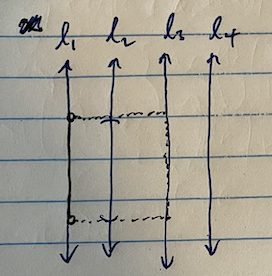
\includegraphics[scale=0.4]{img/1.png}
        \caption{$\ell_1, \ell_2$ intersect the open set at open intervals. $\ell_3, \ell_4$ does not but there are always open sets for which the intersection are open intervals. } 
        \label{fig:1}
      \end{figure}

      \item If $L$ is not vertical, then it is the lower limit topology (or upper limit topology depending on how you parameterize the line). 

      \begin{figure}[H]
        \centering 
        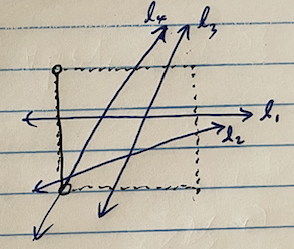
\includegraphics[scale=0.4]{img/2.png}
        \caption{All nonvertical lines will intersect the left ``closed'' side of some open set and will therefore induce the lower/upper limit topology on the line.}
        \label{fig:2}
      \end{figure}
    \end{enumerate}
    The basis of the product topology on $\mathbb{R}_\ell \times \mathbb{R}_\ell$ are all sets of form $[a, b) \times [c, d)$. 
    \begin{enumerate} 
      \item if $L$ has a negative slope (as in the graph represented by $y = mx + b$ where $m < 0$), then it is discrete topology since we can imagine the line intersecting the square at the lower-left corner.\footnote{We can also see it as the topology generated by the basis of closed intervals, but since $[a, b] \cap [b, c] = \{b\}$, this is equivalent to the discrete topology.} 

      \begin{figure}[H]
        \centering 
        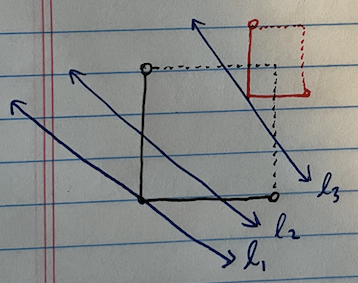
\includegraphics[scale=0.4]{img/3.png}
        \caption{We can construct an open set $[a, b) \times [c, d)$ where the point $(a, c)$ lies on any point on a negatively sloping line. This means that points are open sets, which generates the discrete topology. } 
        \label{fig:3}
      \end{figure}

      \item if $L$ vertical, horizontal, or has a positive slope, then it is the lower limit topology (or upper limit topology depending on how you parameterize the line). 

      \begin{figure}[H]
        \centering 
        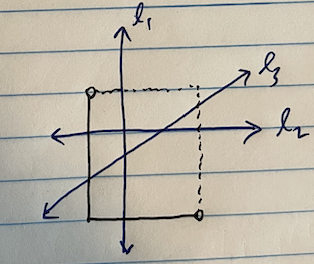
\includegraphics[scale=0.4]{img/4.png}
        \caption{If there is not a negative slope (vertical, horizontal, or positive sloping), then there is no way for a rectangle to intersect the line exactly at the lower-left corner without ``going through'' the rectangle. Therefore these examples generate half-open half-closed intervals on $L$. } 
        \label{fig:4}
      \end{figure}
    \end{enumerate}
  \end{solution}

  \begin{exercise}[Munkres 16.9]
    Show that the dictionary order topology on the set $\mathbb{R} \times \mathbb{R}$ is the same as the product topology $\mathbb{R}_d \times \mathbb{R}$, where $\mathbb{R}_d$ denotes $\mathbb{R}$ in the discrete topology. Compare this topology with the standard topology on $\mathbb{R}^2$.
  \end{exercise}

  \begin{exercise}[Munkres 16.10]
    Let $I = [0, 1]$. Compare the product topology on $I \times I$, the dictionary order topology on $I \times I$, and the topology $I \times I$ inherits as a subspace of $\mathbb{R} \times \mathbb{R}$ in the dictionary order topology.
  \end{exercise}

  \begin{exercise}[Math 411 Spring 2025, PS3]
    Let $P_n$ denote the set of polynomials in n variables with real coefficients. Any such polynomial defines a function on $\mathbb{R}^n$. If A is any subset of $P_n$, let $V(A) = \{x \in \mathbb{R}^n \mid p(x) = 0 \text{ for all } p \in A\}$. A subset $S \subset \mathbb{R}^n$ is called algebraic if it is equal to V(A) for some $A \subset P_n$.

    \begin{enumerate}
      \item Show that $\emptyset$ and $\mathbb{R}^n$ are both algebraic.

      \item Show that if $A_\alpha$ are subsets of $P_n$ (indexed by $\alpha \in I$ for some set I), then
      \[V\left(\bigcup_{\alpha\in I} A_\alpha\right) = \bigcap_{\alpha\in I} V(A_\alpha).\]
      In other words, any intersection of algebraic sets is algebraic.

      \item Suppose $A_1,\ldots,A_k$ are subsets of $P_n$. Let B be the set of polynomials that can be factored as $f = f_1 \cdots f_k$, where $f_i \in A_i$. Prove that
      \[V(B) = V(A_1) \cup \cdots \cup V(A_k).\]
      In other words, any finite union of algebraic sets is algebraic. (Hint: For the inclusion $V(B) \subset V(A_1) \cup \cdots \cup V(A_k)$, it may be easier to show that if $x \not\in V(A_1) \cup \cdots \cup V(A_k)$, then $x \not\in V(B)$.)

      \item Show that $\mathcal{T} = \{U \subset \mathbb{R}^n \mid \mathbb{R}^n - U \text{ is algebraic}\}$ is a topology on $\mathbb{R}^n$. This is known as the Zariski topology, named for the mathematician Oscar Zariski (1899-1986). It is very important in algebraic geometry and related fields.

      \item Show that for n = 1, the Zariski topology on $\mathbb{R}^1$ is precisely the finite complement topology.
    \end{enumerate}

    Note: Instead of doing this with $\mathbb{R}$, you could also do it with $\mathbb{C}$, $\mathbb{Q}$, or any other field.
  \end{exercise}
  \begin{solution}[a]
    Listed. 
    \begin{enumerate}
      \item Consider $A = \{ f(x) = 1\}$. Then $V(A) = \emptyset$ since $f$ never vanishes. 
      \item Consider $A = \{ f(x) = 0 \}$.Then $V(A) = \mathbb{R}^n$ since $f$ always vanishes. 
    \end{enumerate}
  \end{solution}
  \begin{solution}[b]
    We see that 
    \begin{align}
      V \bigg( \bigcup_{\alpha \in I} A_\alpha \bigg) & = \big\{ x \in \mathbb{R}^n \mid \forall p \in \cup_{\alpha \in I} A_\alpha ( p(x) = 0 )\big\} \\ 
                                                      & = \big\{ x \in \mathbb{R}^n \mid \forall \alpha \in I \forall p \in A_\alpha (p(x) = 0)  \big\} \\
                                                      & = \bigcap_{\alpha \in I} \big\{ x \in \mathbb{R}^n \mid \forall p \in A_\alpha (p(x) = 0) \big\} \\
                                                      & = \bigcap_{\alpha \in I} V(A_\alpha)
    \end{align}
  \end{solution}
  \begin{solution}[c]
    We prove bidirectionally. 
    \begin{enumerate}
      \item $\cup_{i} V(A_i) \subset V(B)$. Let $x \in \cup_i V(A_i)$. Then $x \in V(A_j)$ for some $1 \leq j \leq k$, which implies that $f_j (x) = 0$ for all $f_j \in A_j$. Therefore by the field properties of $\mathbb{R}$, 
      \begin{equation}
        f(x) = f_1 (x) \ldots \underbrace{f_j(x)}_{=0} \ldots f_k (x) = 0 
      \end{equation} 
      and therefore $f(x) = 0$ for all $f \in B$, which means that $x \in V(B)$. 

      \item $\cup_i V(A_i) \supset V(B)$. Assume that $x \not\in \cup_i V(A_i)$. Then for all $1 \leq i \leq k$, $x \not\in V(A_i)$, which implies that for all $i$ there exists some $f_i^{\ast} \in A_i$ s.t. $f_i^\ast (x) \neq 0$. Now construct the function $f^\ast = \prod_i f_i^\ast$, where $f_i^\ast \in A_i$, $f^\ast \in B$. But 
      \begin{equation}
        f^\ast (x) = \prod_{i=1}^k f_i^\ast (x) \neq 0
      \end{equation}
      since $f_i^\ast (x) \neq 0$ for all $i$, and so we have shown the existence of a function $f^\ast \in B$ such that $f^\ast (x) \neq 0$. Therefore $x \not\in V(B)$. 
    \end{enumerate}
  \end{solution}
  \begin{solution}[d] 
    We prove the properties of a topology. 
    \begin{enumerate}
      \item From (a), $\emptyset$ is algebraic $\implies \mathbb{R}^n \setminus \emptyset = \mathbb{R}^n$ is in $\mathscr{T}$. Also, $\mathbb{R}^n$ is algebraic $\implies \mathbb{R}^n \setminus \mathbb{R}^n = \emptyset$ is in $\mathscr{T}$.  

      \item Let $\{U_\alpha\}_{\alpha \in I}$ be a collection of open sets in $\mathscr{T}$. Then by definition $\mathbb{R}^n \setminus U_\alpha$ is algebraic, and 
      \begin{equation}
        \mathbb{R}^n \setminus \bigg( \bigcup_{\alpha \in I} U_\alpha \bigg) = \bigcap_{\alpha \in I} (\mathbb{R}^n \setminus U_\alpha) 
      \end{equation} 
      we know from (b) that arbitrary intersections of algebraic sets is algebraic, so the LHS is also algebraic, which by definition means the union is in $\mathscr{T}$. 

      \item Let $U_1, \ldots, U_k$ be a collection of open sets in $\mathscr{T}$. Then by definition $\mathbb{R}^n \setminus U_i$ is algebraic for $1 \leq i \leq k$, and  
      \begin{equation}
        \mathbb{R}^n \setminus \bigg( \bigcap_{i=1}^k U_i \bigg) = \bigcup_{i=1}^k (\mathbb{R}^n \setminus U_i)
      \end{equation}
      we know from (c) that finite unions of algebraic sets is algebraic, and so the LHS is also algebraic, which by definition means the finite intersection is in $\mathscr{T}$. 
    \end{enumerate}
  \end{solution}
  \begin{solution}[e]
    For an open set $U$, inclusion in the finite complement topology asserts that $\mathbb{R} \setminus U$ must be finite or $U = \emptyset$, and inclusion in the Zariski topology asserts that $\mathbb{R} \setminus U$ must be algebraic. Therefore it satisfies to show that the complements (within the universe of the power set) are equal, i.e. that the set of all finite subsets of $\mathbb{R}$ plus $\mathbb{R}$ itself and the set of all algebraic subsets of $\mathbb{R}$ is equal. Let us denote the former $S$ and the latter $T$. 
    \begin{enumerate}
      \item $S \subset T$. Let $Y \in S$ ($Y$ is a set). If $Y = \mathbb{R}$, then it is algebraic as shown in (a). Otherwise, it is finite and we can enumerate it as $Y = \{y_1, \ldots, y_n\}$, and define the singleton subset of polynomials 
      \begin{equation}
        A = \bigg\{ f(x) = \prod_{i=1}^n (x - y_i) \bigg\}
      \end{equation} 
      $V(A)$ consists of all reals where $f(x) = 0$, which happens exactly when $x = y_i$ for some $i$.\footnote{If not, then every $(x - y_i)$ is nonzero, and the product is nonzero.} Therefore, $Y = V(A) \implies Y$ is algebraic $\implies Y \subset T$. 

      \item $T \subset S$. Let $Y \in T$. Then we know that there exists some subset of polynomials $A$ such that $Y = V(A)$. If $A$ is empty, then $V(A) = \mathbb{R}$ since the predicate in the set-builder notation is vacuously true, and $\mathbb{R}$ is contained in the $S$. If $A$ is not empty, then there exists some polynomial $f$ from $A$. By definition it must be the case that for all $y \in Y$, $f(y) = 0$. We consider two cases. 
      \begin{enumerate}
        \item $f$ is constant. If $f \neq 0$, then $V(A) = \emptyset$, which is in $S$. If $f = 0$, then $V(A) = \mathbb{R}$, which is in $S$. 
        \item $f$ has degree $n \geq 1$. Since this is a polynomial ring over a field $\mathbb{F}[x]$, $f(y)$ cannot have more than $n$ real roots.\footnote{Using the single factor theorem of commutative rings we can use induction to prove that the set of roots cannot go beyond $n$. For linear polynomials $f(x) = mx + b$ there is one root $x = -b/m$ which satisfies the base case, and for higher degrees of $n$ we show that if there is a root where $p(a) = 0$, then $p(x) = (x - a) q(x)$ where $q$ is of degree $n-1$ which cannot have more than $n-1$ factors.} Therefore $|Y| \leq n$ and $Y$ must be finite. 
      \end{enumerate}

      We have shown that $V(\{f\})$ is finite. Since $V(A)$ consists of $y$'s that hold for all $f \in A$, $V(A) \subset V(\{f\})$.\footnote{To see why, look at my solution for (b).} The subset of finite sets is finite, and therefore $Y = V(A) \in S$. 
    \end{enumerate}
  \end{solution}

  \begin{exercise}[Munkres 19.4]
    Show that $(X_1 \times \cdots \times X_{n-1}) \times X_n$ is homeomorphic with $X_1 \times \cdots \times X_n$.
  \end{exercise}

  \begin{exercise}[Munkres 19.5]
    One of the implications stated in Theorem 19.6 holds for the box topology. Which one?
  \end{exercise}

  \begin{exercise}[Munkres 19.6]
    Let $\mathbf{x}_1, \mathbf{x}_2, \ldots$ be a sequence of the points of the product space $\prod X_\alpha$. Show that this sequence converges to the point $\mathbf{x}$ if and only if the sequence $\pi_\alpha(\mathbf{x}_1), \pi_\alpha(\mathbf{x}_2), \ldots$ converges to $\pi_\alpha(\mathbf{x})$ for each $\alpha$. Is this fact true if one uses the box topology instead of the product topology?
  \end{exercise}

  \begin{exercise}[Munkres 19.7]
    Let $\mathbb{R}^\infty$ be the subset of $\mathbb{R}^\omega$ consisting of all sequences that are ``eventually zero,'' that is, all sequences $(x_1, x_2, \ldots)$ such that $x_i \neq 0$ for only finitely many values of $i$. What is the closure of $\mathbb{R}^\infty$ in $\mathbb{R}^\omega$ in the box and product topologies? Justify your answer.
  \end{exercise}
  \begin{solution}
    In the box topology, $\overline{\mathbb{R}^\infty} = \mathbb{R}^\infty$. We show this by taking any sequence not in $\mathbb{R}^\infty$ and showing that there exists an open neighborhood that has a trivial intersection with $\mathbb{R}^\infty$. Consider a non-eventually zero sequence $y \in \mathbb{R}^\omega \setminus \mathbb{R}^\infty$, which must have an infinite number of nonzero terms. $y$ is contained within the open set (in the box topology) 
    \begin{equation}
      U = U_1 \times U_2 \times \ldots, \qquad U_i = 
      \begin{cases}
        (0, +\infty) & \text{ if } y_i > 0 \\
        (-1, 1)  & \text{ if } y_i = 0 \\
        (-\infty, 0) & \text{ if } y_i < 0
      \end{cases}
    \end{equation}
    This is an open set that clearly contains $y$, but it has an empty intersection with $\mathbb{R}^\omega$ since there are an infinite number of nonzero terms $y_i$ and so there are an infinite number of $U_i$'s that do not contain $0$. 

    In the product topology, basis elements are all sets of the form $\prod U_i$ where $U_i$ is open in $\mathbb{R}$ and $U_i = \mathbb{R}$ except for finitely many values of $i$. Therefore, $U_i \neq \mathbb{R}$ for finite values. Now given any sequence $y \in \mathbb{R}^\omega$, we claim that it is a limit point of $\mathbb{R}^\infty$. An open neighborhood of $y$ of form $U_y = \prod U_i$ must have some maximum index $N$ for which $U_i = \mathbb{R}$ when $i > N$, and so the eventually-zero sequence $x = (y_1, y_2, \ldots, y_N, 0, 0 ,\ldots)$ must be in $U$, implying that $U_y \cap \mathbb{R}^\infty \neq \emptyset$, and so $y$ is a limit point of $U_y$. Therefore all sequences are limit points, which means $\overline{\mathbb{R}^\infty} = \mathbb{R}^\omega$. 
  \end{solution}

  \begin{exercise}[Munkres 19.8]
    Given sequences $(a_1, a_2, \ldots)$ and $(b_1, b_2, \ldots)$ of real numbers with $a_i > 0$ for all $i$, define $h : \mathbb{R}^\omega \to \mathbb{R}^\omega$ by the equation
    \begin{equation}
      h((x_1, x_2, \ldots)) = (a_1x_1 + b_1, a_2x_2 + b_2, \ldots).
    \end{equation}
    Show that if $\mathbb{R}^\omega$ is given the product topology, $h$ is a homeomorphism of $\mathbb{R}^\omega$ with itself. What happens if $\mathbb{R}^\omega$ is given the box topology?
  \end{exercise}
  \begin{solution}
    We first show $h$ is a bijection. Indeed, the element-wise mappings are bijections and the inverse is 
    \begin{equation}
      h^{-1} ((x_1, \ldots, )) = \bigg(\ldots,  \frac{x_i - b_i}{a_i}, \ldots \bigg)
    \end{equation} 
    Now we show that it is continuous. Given an open set in $\mathbb{R}^\omega$ in the product topology, it has the form 
    \begin{equation}
      U = (l_1, u_1) \times (l_2, u_2) \times \ldots \times (l_n, u_n) \times \mathbb{R} \times \ldots 
    \end{equation} 
    The preimage under $h$ is 
    \begin{equation}
      h^{-1} (U) = \bigg( \frac{l_1 - b_1}{a_1}, \frac{u_1 - b_1}{a_1} \bigg) \times \ldots \times \bigg( \frac{l_n - b_n}{a_n}, \frac{u_n - b_n}{a_n} \bigg) \times \mathbb{R} \times \ldots
    \end{equation}
    where $l_1 < u_1 \implies (l_1 - b_1) /a_1 < (u_1 - b_1) / a_1$. This is also of the form of open sets in the product topology, and therefore is continuous. Now considering the continuity of the inverse function, we can see that taking the same $U$ as before, we have 
    \begin{equation}
      h(U) = (a_1 l_1 + b_1, a_1 u_1 + b_1) \times \ldots \times (a_n l_n + b_n, a_n u_n + b_n) \times \mathbb{R} \ldots 
    \end{equation}
    which is also open in the product topology. Therefore $h$ is a homeomorphism under the product topologies. 

    Now we consider the box topology. Given an box-topology open set of the form 
    \begin{equation}
      U = (l_1, u_1) \times (l_2, u_2) \times \ldots
    \end{equation} 
    then the preimage and image are 
    \begin{align}
      h^{-1} (U) & = \bigg( \frac{l_1 - b_1}{a_1}, \frac{u_1 - b_1}{a_1} \bigg) \times \bigg( \frac{l_2 - b_2}{a_2}, \frac{u_2 - b_2}{a_2} \bigg) \times \ldots \\
      h(U) & = h(U) = (a_1 l_1 + b_1, a_1 u_1 + b_1) \times (a_2 l_2 + b_2, a_2 u_2 + b_2) \times 
    \end{align}
    which are both open in the box topology and so $h$ and $h^{-1}$ are continuous. Thus $h$ is also a homeomorphism. 
  \end{solution}

  \begin{exercise}[Munkres 19.9]
    Show that the choice axiom is equivalent to the statement that for any indexed family $\{A_\alpha\}_{\alpha \in J}$ of nonempty sets, with $J \neq \emptyset$, the cartesian product
    \begin{align*}
      \prod_{\alpha \in J} A_\alpha
    \end{align*}
    is not empty.
  \end{exercise}

  \begin{exercise}[Munkres 19.10]
    Let $A$ be a set; let $\{X_\alpha\}_{\alpha \in J}$ be an indexed family of spaces; and let $\{f_\alpha\}_{\alpha \in J}$ be an indexed family of functions $f_\alpha : A \to X_\alpha$.
    \begin{enumerate}
      \item Show there is a unique coarsest topology $\mathcal{T}$ on $A$ relative to which each of the functions $f_\alpha$ is continuous.
      \item Let
      \begin{align*}
        S_\beta = \{f_\beta^{-1}(U_\beta) \mid U_\beta \text{ is open in } X_\beta\},
      \end{align*}
      and let $S = \bigcup S_\beta$. Show that $S$ is a subbasis for $\mathcal{T}$.
      \item Show that a map $g : Y \to A$ is continuous relative to $\mathcal{T}$ if and only if each map $f_\alpha \circ g$ is continuous.
      \item Let $f : A \to \prod X_\alpha$ be defined by the equation
      \begin{align*}
        f(a) = (f_\alpha(a))_{\alpha \in J};
      \end{align*}
      let $Z$ denote the subspace $f(A)$ of the product space $\prod X_\alpha$. Show that the image under $f$ of each element of $\mathcal{T}$ is an open set of $Z$.
    \end{enumerate}
  \end{exercise}

  \begin{exercise}[Munkres 22.2]
    \begin{enumerate}
      \item[(a)] Let $p : X \to Y$ be a continuous map. Show that if there is a continuous map
        $f : Y \to X$ such that $p \circ f$ equals the identity map of $Y$, then $p$ is a quotient
        map.
      
      \item[(b)] If $A \subset X$, a \textit{retraction} of $X$ onto $A$ is a continuous map $r : X \to A$ such
        that $r(a) = a$ for each $a \in A$. Show that a retraction is a quotient map.
    \end{enumerate}
  \end{exercise}
  \begin{solution}
     Listed. 
     \begin{enumerate}
       \item Let $U \subset Y$, and let $p^{-1}(U)$ be open. Then, 
       \begin{align}
         p^{-1} (U) \subset X \text{ open} & \implies f^{-1} (p^{-1}(U)) \subset Y \text{ open} \\
                                           & \implies (p \circ f)^{-1} (U) = U \subset Y \text{ open}
       \end{align}
       and since $p$ is continuous, $p$ is a quotient map. Since $p \circ f$ equals the identity map, it must be the case that $p$ is surjective. 

       \item We know that the canonical injection $\iota: A \rightarrow X$ is continuous, and $r \circ \iota = I$, the identity map of $A$. Therefore by (a), $p$ is a quotient map. 
     \end{enumerate}
  \end{solution}

  \begin{exercise}[Munkres 22.3]
    Let $\pi_1 : \mathbb{R} \times \mathbb{R} \to \mathbb{R}$ be projection on the first coordinate. Let $A$ be the subspace of $\mathbb{R} \times \mathbb{R}$ consisting of all points $x \times y$ for which either $x \geq 0$ or $y = 0$ (or both); let $q : A \to \mathbb{R}$ be obtained by restricting $\pi_1$. Show that $q$ is a quotient map that is neither open nor closed.
  \end{exercise}
  \begin{solution} 
    The restriction of a continuous function is always continuous, so $q$ is continuous. Furthermore $q$ is surjective since given any $x \in \mathbb{R}$, we can always see that $(x, 0) \in q^{-1}(\{x\})$. Finally, let $U \subset \mathbb{R}$ s.t. $q^{-1} (U) \subset A$ is open. Then, for any $x \in U$, we know $(x, 0) \subset q^{-1} (U)$, and so  $\exists \epsilon > 0$ s.t. $B((x, 0), \epsilon) \cap A) \subset q^{-1} (U)$. Mapping both sides through $q$ again gives 
    \begin{equation}
      (x - \epsilon, x + \epsilon) = q\big( B((x, 0), \epsilon) \cap A) \big) \subset q (q^{-1}(U)) = U
    \end{equation}
    and so $U$ is open. Therefore, $q$ is a quotient map. To see why it is not open, consider the open set of $A$ 
    \begin{equation}
      U = [0, 1) \times (0, 1) = [(-1, 1) \times (0, 1)] \cap A 
    \end{equation} 
    Then $q(U) = [0, 1)$ which is not open in $\mathbb{R}$. To see why not closed, consider the closed set $C = \{(x, y) \in \mathbb{R}^2 \mid xy = 1, x > 0 \}$.\footnote{Also stated to be closed by example 2 of chapter 22.} Then $p(C) = (0, +\infty)$ which is not closed in $\mathbb{R}$. 
  \end{solution}

  \begin{exercise}[Munkres 22.4]
    \begin{enumerate}
      \item[(a)] Define an equivalence relation on the plane $X = \mathbb{R}^2$ as follows:
      \begin{center}
        $x_0 \times y_0 \sim x_1 \times y_1$ \quad if $x_0 + y_0^2 = x_1 + y_1^2$.
      \end{center}
      Let $X^*$ be the corresponding quotient space. It is homeomorphic to a familiar
      space; what is it? 
      
      \item[(b)] Repeat (a) for the equivalence relation
      \begin{center}
        $x_0 \times y_0 \sim x_1 \times y_1$ \quad if $x_0^2 + y_0^2 = x_1^2 + y_1^2$.
      \end{center}
    \end{enumerate}
  \end{exercise}
  \begin{solution}
    Listed. 
    \begin{enumerate}
      \item Graphing this shows that $X^\ast$ is the set of all horizontal parabolas of the same scale and opening leftwards with the vertex on the $x$-axis, i.e. the elements are just left-right shifts of one another. We claim that it is homeomorphic to $\mathbb{R}$. Let $p: \mathbb{R}^2 \rightarrow X^\ast$ be the quotient map and $f: \mathbb{R}^2 \rightarrow \mathbb{R}$ be defined $f(x, y) = x + y^2$, which satisfies $(x,y) \sim (x^\prime, y^\prime) \iff f(x, y) = f(x^\prime, y^\prime)$. Therefore, this induces a function $\bar{f}: X^\ast  \rightarrow \mathbb{R}$ s.t. $\bar{f} \circ p = f$. Since $f$ is continuous, $\bar{f}$ is continuous. Also, we can see that $\bar{f}$ is a bijection since we can map every element in the equivalence class of $[(x, y)]$ s.t. $x + y^2 = c$ to $c \in \mathbb{R}$. Finally, we show that $\bar{f}^{-1}$ is continuous. We can think of $\bar{f}^{-1}$ as the composition of maps $c \mapsto (c, 0) \mapsto [(c, 0)]$, where the first map is trivially continuous and the second map is $p$, which is also continuous. Therefore $\bar{f}^{-1}$ is continuous, and it is a homeomorphism. 
        
      \item We can see that $X^\ast$ is the set of all circles of nonnegative radius (the origin is a circle of radius $0$), and we claim that it is homeomorphic to $[0, +\infty)$. Let $p: \mathbb{R}^2 \rightarrow X^\ast$ be the quotient map and $f: \mathbb{R}^2 \rightarrow [0, +\infty)$ be defined $f(x, y) = x^2 + y^2$, which satisfies $(x,y) \sim (x^\prime, y^\prime) \iff f(x, y) = f(x^\prime, y^\prime)$. Therefore, this induces a function $\bar{f}: X^\ast  \rightarrow [0, +\infty)$ s.t. $\bar{f} \circ p = f$. Since $f$ is continuous, $\bar{f}$ is continuous. Also, we can see that $\bar{f}$ is a bijection since we can map every element in the equivalence class of $[(x, y)]$ s.t. $x^2 + y^2 = c$ to $c \in [0, +\infty)$. Finally, we show that $\bar{f}^{-1}$ is continuous. We can think of $\bar{f}^{-1}$ as the composition of maps $c \mapsto (\sqrt{c}, 0) \mapsto [(\sqrt{c}, 0)]$, where the first map is continuous\footnote{The square root function from $\mathbb{R}_0^+$ to itself is continuous since the preimage of an open interval $(a, b)$ is $(\sqrt{a}, \sqrt{b})$ which is also open in $\mathbb{R}_0^+$, and for $[0, b)$ the preimage is $[0, \sqrt{b})$.} and the second map is $p$, which is also continuous. Therefore $\bar{f}^{-1}$ is continuous, and it is a homeomorphism. 
    \end{enumerate}
  \end{solution}

  \begin{exercise}[Munkres 22.5]
    Let $p : X \to Y$ be an open map. Show that if $A$ is open in $X$, then the map $q : A \to p(A)$ obtained by restricting $p$ is an open map.
  \end{exercise}

  \begin{exercise}[Munkres 22.6]
    Recall that $\mathbb{R}_K$ denotes the real line in the $K$-topology. (See \S13.) Let $Y$ be the quotient space obtained from $\mathbb{R}_K$ by collapsing the set $K$ to a point; let $p : \mathbb{R}_K \to Y$ be the quotient map.
    \begin{enumerate} 
      \item[(a)] Show that $Y$ satisfies the $T_1$ axiom, but is not Hausdorff.
      \item[(b)] Show that $p \times p : \mathbb{R}_K \times \mathbb{R}_K \to Y \times Y$ is not a quotient map. [Hint: The diagonal is not closed in $Y \times Y$, but its inverse image is closed in $\mathbb{R}_K \times \mathbb{R}_K$.]
    \end{enumerate}
  \end{exercise}

  \begin{exercise}[Math 411 Spring 2025, PS6]
    For each integer $n \geq 1$, let us consider the following spaces:
    \begin{align*}
      S^n &= \{\mathbf{x} \in \mathbb{R}^{n+1} \mid \|\mathbf{x}\|= 1\} \\
      X^{n+1} &= \mathbb{R}^{n+1} - \{\mathbf{0}\}
    \end{align*}
    (Note: the superscript is just a decoration that indicates the ``dimensionality''
    of the space; it does \textit{not} indicate raising something to a power.)
    \begin{enumerate}
      \item[(1)] Show that the function $r : X^{n+1} \to S^n$ defined by $r(\mathbf{x}) = \mathbf{x}/\|\mathbf{x}\|$ is a
        quotient map, and describe the corresponding equivalence relation. (Hint:
        Use \#2 from \S22.)
        
      \item[(2)] We now define a space called \textit{real projective n-space}, or $\mathbb{RP}^n$. We can
        define it in either of two ways:
        \begin{enumerate}
          \item[(a)] $X^{n+1}/{\sim}$, where $\mathbf{x} \sim \mathbf{y}$ iff $\mathbf{x} = \lambda\mathbf{y}$ for some $\lambda \in \mathbb{R} - \{0\}$.
          \item[(b)] $S^n/{\sim}$, where $\mathbf{x} \sim \mathbf{y}$ iff $\mathbf{x} = \pm\mathbf{y}$.
        \end{enumerate}
        Let $p : X^{n+1} \to \mathbb{RP}^n$ be the quotient map. Prove that $p|_{S^n} : S^n \to \mathbb{RP}^n$ is
        also a quotient map, and hence that the two descriptions above produce
        homeomorphic spaces. (Hint: It may help to observe that $p|_{S^n} \circ r = p$.)
        
      \item[(3)] Using the description of $\mathbb{RP}^n$ as a quotient of $S^n$, prove that $\mathbb{RP}^n$ is
        a Hausdorff space. (Hint: note that for $\mathbf{x} \in S^n$ and $\epsilon > 0$, the set
        $(B(\mathbf{x},\epsilon) \cup B(-\mathbf{x},\epsilon)) \cap S^n$ is open and saturated.)
        
      \item[(4)] Let $D^n_+$ denote the ``upper hemisphere'' in $S^n$: $D^n_+ = \{\mathbf{x} \in S^n \mid x_{n+1} \geq 0\}$.
        Show that $D^n_+$ is homeomorphic to $D^n = \{\mathbf{x} \in \mathbb{R}^n \mid \|\mathbf{x}\| \leq 1\}$, the unit
        disk in $\mathbb{R}^n$.
        
      \item[(5)] The restriction of $p$ to $D^n$, viewed as a map $D^n \to \mathbb{RP}^n$, can be shown
        to be a quotient map. Assuming this, describe an equivalence relation
        on $D^n$ whose quotient space is homeomorphic to $\mathbb{RP}^n$. In the case where
        $n = 2$, describe how we may concretely describe $\mathbb{RP}^2$ as a ``video game.''
    \end{enumerate}
  \end{exercise}
  \begin{solution}
    Listed. 
    \begin{enumerate}
      \item We claim $r$ is a retraction, since $r(x) = x$ for all $x \in S^n \subset \mathbb{R}^{n+1}$. $r$ is also continuous since a basis element of the topology of $S^n$ can be written $B = \big\{(a_1, b_1) \times \ldots \times (a_{n+1}, b_{n+1}) \big\} \cap S^n$. Therefore the preimage of such a set is 
      \begin{equation}
        r^{-1} (B) = \bigcup_{c > 0} \big\{(c a_1, c b_1) \times \ldots \times (c a_{n+1}, c b_{n+1}) \big\} \cap S^n 
      \end{equation}
      which is the union of open sets in $S^n$ and therefore is open in $S^n$. From the first exercise, $r$ is a quotient map. It consists of each ray starting from the origin, and maps each direction to the unit vector, creating a sphere.   


      \item $p|_{S^n} \circ r = p$. Since $p$ is a quotient map, it is continuous and its restriction $p|_{S^n}$ is also continuous. Since $p$ is a quotient map, it is surjective and therefore $p|_{S^n}$ must be surjective.\footnote{If $p|_{S^n}$ wasn't surjective, then $p|_{S^n} \circ r$ is not surjective and $p$ is not surjective, a contradiction. } Now let $U \subset \mathbb{RP}^n$ s.t. $p|_{S^n}^{-1} (U)$ is open in $S^n$. Then, 
      \begin{equation}
        r^{-1} \big( p|_{S^n}^{-1} (U) \big) = (p |_{S^n} \circ r)^{-1} (U) = p^{-1} (U)
      \end{equation} 
      is open since $r$ is continuous. But since $p$ is a quotient map, $U$ is open, implying that $p|_{S^n}$ is a quotient map. Therefore, we have shown that 
      \begin{equation}
        X^{n+1} / \sim \cong \mathbb{RP}^n \text{ and } S^n / \sim \cong \mathbb{RP}^n \implies X^{n+1} / \sim \cong S^n / \sim
      \end{equation}

      \item Let us have $x, y \in \mathbb{RP}^n$ with $x \neq y$. Then there exists $u, v \in S^n$ s.t. $p|_{S^n}^{-1}(x) = \{u, -u\}$ and $p|_{S^n}^{-1} (y) = \{v, -v\}$. We can let $\epsilon = \frac{1}{2} \min\{ \|u - v\|, \|u + v\|\}$, which means that 
      \begin{equation}
        B(\pm u, \epsilon) \cap B(\pm v, \epsilon) = \emptyset 
      \end{equation}
      in $\mathbb{R}^n$, and so the open neighborhoods around $\pm u, \pm v$, denoted $U_{\pm}, V_{\pm}$ are all pairwise disjoint in $S^n$. Note that $U_+ \cup U_-$ and $V_+ \cup V_-$ are open, saturated, and disjoint, and so $p|_{S^n}$, as a quotient map, maps both of these sets to disjoint open neighborhoods of $x, y$, proving that $\mathbb{RP}^n$ is Hausdorff. 

      \item We can visualize this as if we were just ``pushing up'' the disk onto the hemisphere. More formally, let us define $f: D^n \rightarrow D_+^n$ as 
      \begin{equation}
        f(x) = f(x_1, \ldots, x_n) = (x_1, \ldots, x_n, \sqrt{1 - \|x\|})
      \end{equation}
      This is well-defined since we assume that $\|x\| \leq 1$. This is trivially injective since changing any of the $x_i$'s will result in a different values in the first $n$ terms of the output. It is surjective since given any element $y = (y_1, \ldots, y_{n+1}) \in D_+$, we know that $\|y\| = 1$ and so we can find the preimage to be $x = (y_1, \ldots, y_n)$ which will satisfy $\|x\| \leq 1$. Therefore, $f$ is bijective, with the inverse function 
      \begin{equation}
        f^{-1} (y) = f^{-1} (y_1, \ldots, y_{n+1}) = (y_1, \ldots, y_{n})
      \end{equation}
      To prove continuity of $f$, consider the basis element of the form 
      \begin{equation}
        (a_1, b_1) \times \ldots \times (a_{n+1}, b_{n+1}) \cap D_+^n 
      \end{equation}
      the preimage is 
      \begin{equation}
        f^{-1} \big( (a_1, b_1) \times \ldots \times (a_{n+1}, b_{n+1})\big) \cap f^{-1} (D_+^n) = (a_1, b_1) \times (a_n, b_n) \cap D^n 
      \end{equation}
      which is a basis element of $D^n$. To prove continuity of $f^{-1}$, we consider its extension $f^{-1}: \mathbb{R}^{n+1} \rightarrow \mathbb{R}^n$, which is simply a projection of the first $n$ elements and is therefore continuous. The restriction of this function $f^{-1}: D_+^n \rightarrow \mathbb{R}^n$ is therefore continuous, and since the image of $f^{-1}$ only hits $D^n$, every open set in $D^n$ is of the form $U = V \cap D^n$ for $V$ open in $\mathbb{R}^n$, where the preimage will simply be $f(U) = f(V) \cap f(D^n)$. We know $f(V)$ is open\footnote{by continuity of $f^{-1}$ with codomain $\mathbb{R}^n$} and $f(D^n) = D^n_+$, $f(U)$ is open in $D_+^n$. 

      \item In $D^n$, we define the equivalence relation $\sim$ where $x \sim -x$ if $\|x\| = 1$, and every other point (in the interior of the disk) is equivalent to itself only. When $n=2$, we can imagine a player walking in a circular disk in $\mathbb{R}^2$, and when it crosses the boundary it will end up at the antipodal point. 
    \end{enumerate}
  \end{solution}

\subsection{Metric Topologies}

  \begin{exercise}[Munkres 20.1]
    \begin{enumerate} 
      \item[(a)] In $\mathbb{R}^n$, define
      \begin{align*}
        d'(\mathbf{x}, \mathbf{y}) = |x_1 - y_1| + \cdots + |x_n - y_n|.
      \end{align*}
      Show that $d'$ is a metric that induces the usual topology of $\mathbb{R}^n$. Sketch the basis elements under $d'$ when $n = 2$.
      
      \item[(b)] More generally, given $p \geq 1$, define
      \begin{align*}
        d'(\mathbf{x}, \mathbf{y}) = \left[\sum_{i=1}^{n} |x_i - y_i|^p\right]^{1/p}
      \end{align*}
      for $\mathbf{x}, \mathbf{y} \in \mathbb{R}^n$. Assume that $d'$ is a metric. Show that it induces the usual topology on $\mathbb{R}^n$.
    \end{enumerate}
  \end{exercise}

  \begin{exercise}[Munkres 20.2]
    Show that $\mathbb{R} \times \mathbb{R}$ in the dictionary order topology is metrizable.
  \end{exercise}

  \begin{exercise}[Munkres 20.3]
    \begin{enumerate} 
      \item[(a)] Let $X$ be a metric space with metric $d$. Show that $d : X \times X \to \mathbb{R}$ is continuous.
      
      \item[(b)] Let $X'$ denote a space having the same underlying set as $X$. Show that if $d : X' \times X' \to \mathbb{R}$ is continuous, then the topology of $X'$ is finer than the topology of $X$.
    \end{enumerate}
    
    One can summarize the result of this exercise as follows: If $X$ has a metric $d$, then the topology induced by $d$ is the coarsest topology relative to which the function $d$ is continuous.
  \end{exercise}

  \begin{exercise}[Munkres 20.4]
    Consider the product, uniform, and box topologies on $\mathbb{R}^\omega$.
    \begin{enumerate} 
      \item[(a)] In which topologies are the following functions from $\mathbb{R}$ to $\mathbb{R}^\omega$ continuous?
      \begin{align*}
        f(t) &= (t, 2t, 3t, \ldots), \\
        g(t) &= (t, t, t, \ldots), \\
        h(t) &= (t, \frac{1}{2}t, \frac{1}{3}t, \ldots).
      \end{align*}
      
      \item[(b)] In which topologies do the following sequences converge?
      \begin{align*}
        \mathbf{w}_1 &= (1, 1, 1, 1, \ldots), & \mathbf{x}_1 &= (1, 1, 1, 1, \ldots), \\
        \mathbf{w}_2 &= (0, 2, 2, 2, \ldots), & \mathbf{x}_2 &= (0, \frac{1}{2}, \frac{1}{2}, \frac{1}{2}, \ldots), \\
        \mathbf{w}_3 &= (0, 0, 3, 3, \ldots), & \mathbf{x}_3 &= (0, 0, \frac{1}{3}, \frac{1}{3} \ldots), \\
        \ldots & & \ldots \\
        \mathbf{y}_1 &= (1, 0, 0, 0, \ldots), & \mathbf{z}_1 &= (1, 1, 0, 0, \ldots), \\
        \mathbf{y}_2 &= (\frac{1}{2}, \frac{1}{2}, 0, 0, \ldots), & \mathbf{z}_2 &= (\frac{1}{2}, \frac{1}{2}, 0, 0, \ldots), \\
        \mathbf{y}_3 &= (\frac{1}{3}, \frac{1}{3}, \frac{1}{3}, 0, \ldots), & \mathbf{z}_3 &= (\frac{1}{3}, \frac{1}{3}, 0, 0, \ldots), \\
        \ldots & & \ldots
      \end{align*}
    \end{enumerate}
  \end{exercise}

  \begin{exercise}[Munkres 20.5]
    Let $\mathbb{R}^\infty$ be the subset of $\mathbb{R}^\omega$ consisting of all sequences that are eventually zero. What is the closure of $\mathbb{R}^\infty$ in $\mathbb{R}^\omega$ in the uniform topology? Justify your answer.
  \end{exercise}

  \begin{exercise}[Munkres 20.6]
    Let $\bar{\rho}$ be the uniform metric on $\mathbb{R}^\omega$. Given $\mathbf{x} = (x_1, x_2, \ldots) \in \mathbb{R}^\omega$ and given $0 < \epsilon < 1$, let
    \begin{align*}
      U(\mathbf{x}, \epsilon) = (x_1 - \epsilon, x_1 + \epsilon) \times \cdots \times (x_n - \epsilon, x_n + \epsilon) \times \cdots.
    \end{align*}
    \begin{enumerate} 
      \item[(a)] Show that $U(\mathbf{x}, \epsilon)$ is not equal to the $\epsilon$-ball $B_{\bar{\rho}}(\mathbf{x}, \epsilon)$.
      \item[(b)] Show that $U(\mathbf{x}, \epsilon)$ is not even open in the uniform topology.
      \item[(c)] Show that
      \begin{align*}
        B_{\bar{\rho}}(\mathbf{x}, \epsilon) = \bigcup_{\delta < \epsilon} U(\mathbf{x}, \delta).
      \end{align*}
    \end{enumerate}
  \end{exercise}

  \begin{exercise}[Munkres 20.7]
    Consider the map $h : \mathbb{R}^\omega \to \mathbb{R}^\omega$ defined in Exercise 8 of \S19; give $\mathbb{R}^\omega$ the uniform topology. Under what conditions on the numbers $a_i$ and $b_i$ is $h$ continuous? a homeomorphism?
  \end{exercise}

  \begin{exercise}[Munkres 20.8]
    Let $X$ be the subset of $\mathbb{R}^\omega$ consisting of all sequences $\mathbf{x}$ such that $\sum x_i^2$ converges. Then the formula
    \begin{align*}
      d(\mathbf{x}, \mathbf{y}) = \left[\sum_{i=1}^{\infty}(x_i - y_i)^2\right]^{1/2}
    \end{align*}
    defines a metric on $X$. (See Exercise 10.) On $X$ we have the three topologies it inherits from the box, uniform, and product topologies on $\mathbb{R}^\omega$. We have also the topology given by the metric $d$, which we call the $\ell^2$-topology. (Read "little ell two.")
    \begin{enumerate} 
      \item[(a)] Show that on $X$, we have the inclusions
      \begin{align*}
        \text{box topology} \supset \ell^2\text{-topology} \supset \text{uniform topology}.
      \end{align*}
      
      \item[(b)] The set $\mathbb{R}^\infty$ of all sequences that are eventually zero is contained in $X$. Show that the four topologies that $\mathbb{R}^\infty$ inherits as a subspace of $X$ are all distinct.
      
      \item[(c)] The set
      \begin{align*}
        H = \prod_{n\in\mathbb{Z}_+} [0, 1/n]
      \end{align*}
      is contained in $X$; it is called the Hilbert cube. Compare the four topologies that $H$ inherits as a subspace of $X$.
    \end{enumerate}
  \end{exercise}

  \begin{exercise}[Munkres 20.9]
    Show that the euclidean metric $d$ on $\mathbb{R}^n$ is a metric, as follows: If $\mathbf{x}, \mathbf{y} \in \mathbb{R}^n$ and $c \in \mathbb{R}$, define
    \begin{align*}
      \mathbf{x} + \mathbf{y} &= (x_1 + y_1, \ldots, x_n + y_n), \\
      c\mathbf{x} &= (cx_1, \ldots, cx_n), \\
      \mathbf{x} \cdot \mathbf{y} &= x_1y_1 + \cdots + x_ny_n.
    \end{align*}
    \begin{enumerate} 
      \item[(a)] Show that $\mathbf{x} \cdot (\mathbf{y} + \mathbf{z}) = (\mathbf{x} \cdot \mathbf{y}) + (\mathbf{x} \cdot \mathbf{z})$.
      \item[(b)] Show that $|\mathbf{x}\cdot\mathbf{y}| \leq \|\mathbf{x}\|\|\mathbf{y}\|$. [Hint: If $\mathbf{x}, \mathbf{y} \neq 0$, let $a = 1/\|\mathbf{x}\|$ and $b = 1/\|\mathbf{y}\|$, and use the fact that $\|a\mathbf{x} \pm b\mathbf{y}\| \geq 0$.]
      \item[(c)] Show that $\|\mathbf{x} + \mathbf{y}\| \leq \|\mathbf{x}\| + \|\mathbf{y}\|$. [Hint: Compute $(\mathbf{x} + \mathbf{y}) \cdot (\mathbf{x} + \mathbf{y})$ and apply (b).]
      \item[(d)] Verify that $d$ is a metric.
    \end{enumerate}
  \end{exercise}

  \begin{exercise}[Munkres 20.10]
    Let $X$ denote the subset of $\mathbb{R}^\omega$ consisting of all sequences $(x_1, x_2, \ldots)$ such that $\sum x_i^2$ converges. (You may assume the standard facts about infinite series. In case they are not familiar to you, we shall give them in Exercise 11 of the next section.)
    \begin{enumerate} 
      \item[(a)] Show that if $\mathbf{x}, \mathbf{y} \in X$, then $\sum |x_i y_i|$ converges. [Hint: Use (b) of Exercise 9 to show that the partial sums are bounded.]
      \item[(b)] Let $c \in \mathbb{R}$. Show that if $\mathbf{x}, \mathbf{y} \in X$, then so are $\mathbf{x} + \mathbf{y}$ and $c\mathbf{x}$.
      \item[(c)] Show that
      \begin{align*}
        d(\mathbf{x}, \mathbf{y}) = \left[\sum_{i=1}^{\infty}(x_i - y_i)^2\right]^{1/2}
      \end{align*}
      is a well-defined metric on $X$.
    \end{enumerate}
  \end{exercise}

  \begin{exercise}[Munkres 20.11]
    Show that if $d$ is a metric for $X$, then
    \begin{align*}
      d'(x, y) = d(x, y)/(1 + d(x, y))
    \end{align*}
    is a bounded metric that gives the topology of $X$. [Hint: If $f(x) = x/(1 + x)$ for $x > 0$, use the mean-value theorem to show that $f(a + b) - f(b) \leq f(a)$.]
  \end{exercise}

  \begin{exercise}[Munkres 21.1]
    Let $A \subset X$. If $d$ is a metric for the topology of $X$, show that $d|A \times A$ is a metric for the subspace topology on $A$.
  \end{exercise}

  \begin{exercise}[Munkres 21.2]
    Let $X$ and $Y$ be metric spaces with metrics $d_X$ and $d_Y$, respectively. Let $f : X \to Y$ have the property that for every pair of points $x_1, x_2$ of $X$,
    \begin{align*}
      d_Y(f(x_1), f(x_2)) = d_X(x_1, x_2).
    \end{align*}
    Show that $f$ is an imbedding. It is called an \textit{isometric imbedding} of $X$ in $Y$.
  \end{exercise}

  \begin{exercise}[Munkres 21.3]
    Let $X_n$ be a metric space with metric $d_n$, for $n \in \mathbb{Z}_+$.
    \begin{enumerate}
      \item Show that
        \begin{equation}
          \rho(x,y) = \max\{d_1(x_1, y_1), \ldots, d_n(x_n, y_n)\}
        \end{equation}
        is a metric for the product space $X_1 \times \cdots \times X_n$.
      
      \item Let $\tilde{d_i} = \min\{d_i, 1\}$. Show that
        \begin{equation}
          D(x,y) = \sup\{\tilde{d_i}(x_i, y_i)/i\}
        \end{equation}
        is a metric for the product space $\prod X_i$.
    \end{enumerate}
  \end{exercise}
  \begin{solution}
    For the first part, we prove the properties of the metric. 
    \begin{enumerate}
      \item Nonnegativity. Note that $\rho$ is the maximum of a finite set of metrics, which must be nonnegative, and so $\rho(x, y) \geq 0$. Second,  
      \begin{align}
        \rho(x, y) = 0 & \iff \max\{d_i (x_i, y_i)\} = 0 \\
                       & \iff d_i (x_i, y_i) = 0 \text{ for all } i = 1, \ldots, n  \\
                       & \iff x_i = y_i \text{ for all } i \\
                       & \iff x = y
      \end{align}

      \item Symmetricity. 
      \begin{equation}
        \rho(x, y) = \max\{d_i (x_i, y_i)\} = \max\{d_i (y_i, x_i)\} = \rho(y, x)
      \end{equation}

      \item Triangle inequality. 
      \begin{align}
        \rho(x, y) + \rho(y, z) & = \max_i \{d_i (x_i, y_i)\} + \max_j \{d_j (y_j, z_j)\} \\
                                & \geq \max_i \{ d_i (x_i, y_i) + d_i (y_i, z_i) \} \\
                                & \geq \max_i \{ d_i (x_i, z_i) \} \\
                                & = \rho(x, z)
      \end{align}
    \end{enumerate} 
    
    For the second part, we do the same. 
    \begin{enumerate}
      \item Nonnegativity. Since $\tilde{d}_i \geq 0$, $\tilde{d}_i / i \geq 0/i = 0$ and so the supremum must be at least $0$ (if it's negative then it will not bound $d_1$.) Second, 
        \begin{align}
          D(x, y) = 0 & \iff \sup\{\tilde{d}_i (x_i, y_i) / i \} = 0 \\
                      & \iff \tilde{d}_i (x_i, y_i) / i = 0 \text{ for all } i \\
                      & \iff \tilde{d}_i (x_i, y_i) = 0 \text{ for all } i \\
                      & \iff \min\{d_i (x_i, y_i), 1 \} = 0 \text{ for all } i \\ 
                      & \iff d_i (x_i, y_i) = 0 \text{ for all } i \\
                      & \iff x_i = y_i \text{ for all } i \\
                      & \iff x = y
        \end{align}

      \item Symmetricity. 
        \begin{equation}
          D(x, y) = \sup\{\tilde{d}_i (x_i, y_i) / i \} = \sup\{\tilde{d}_i (y_i, x_i) / i \} = D(y, x)
        \end{equation}

      \item Triangle inequality. 
        \begin{align}
          D(x, y) + D(y, z) & = \sup_i \{\tilde{d}_i (x_i, y_i) / i \} + \sup_j \{\tilde{d}_j (y_j, z_j) / j \} \\
                            & \geq \sup_i \bigg\{ \frac{\tilde{d}_i (x_i, y_i) + \tilde{d}_i (y_i, z_i)}{i} \bigg\} \\
                            & = \sup_i \bigg\{ \frac{ \min\{d_i (x_i, y_i), 1\} + \min\{ d_i (y_i, z_i), 1\}}{i} \bigg\} \\
                            & \geq \sup_i \bigg\{ \frac{ \min\{d_i (x_i, y_i) + d_i (y_i, z_i), 1\}}{i} \bigg\} \\ 
                            & \geq \sup_i \bigg\{ \frac{ \min\{d_i (x_i, z_i), 1\}}{i} \bigg\} \\ 
                            & = D(x, z)
        \end{align}
    \end{enumerate}
  \end{solution}

  \begin{exercise}[Munkres 21.4]
    Show that $\mathbb{R}_\ell$ and the ordered square satisfy the first countability axiom. (This result does not, of course, imply that they are metrizable.)
  \end{exercise}

  \begin{exercise}[Munkres 21.5]
    Theorem. Let $x_n \to x$ and $y_n \to y$ in the space $\mathbb{R}$. Then
    \begin{align*}
      x_n + y_n &\to x + y, \\
      x_n - y_n &\to x - y, \\
      x_ny_n &\to xy,
    \end{align*}
    and provided that each $y_n \neq 0$ and $y \neq 0$,
    \begin{align*}
      x_n/y_n \to x/y.
    \end{align*}
    [Hint: Apply Lemma 21.4; recall from the exercises of \S19 that if $x_n \to x$ and $y_n \to y$, then $x_n \times y_n \to x \times y$.]
  \end{exercise}

  \begin{exercise}[Munkres 21.6]
    Define $f_n : [0, 1] \to \mathbb{R}$ by the equation $f_n(x) = x^n$. Show that the sequence $(f_n(x))$ converges for each $x \in [0, 1]$, but that the sequence $(f_n)$ does not converge uniformly.
  \end{exercise}

  \begin{exercise}[Munkres 21.7]
    Let $X$ be a set, and let $f_n : X \to \mathbb{R}$ be a sequence of functions. Let $\bar{\rho}$ be the uniform metric on the space $\mathbb{R}^X$. Show that the sequence $(f_n)$ converges uniformly to the function $f : X \to \mathbb{R}$ if and only if the sequence $(f_n)$ converges to $f$ as elements of the metric space $(\mathbb{R}^X, \bar{\rho})$.
  \end{exercise}

  \begin{exercise}[Munkres 21.8]
    Let $X$ be a topological space and let $Y$ be a metric space. Let $f_n : X \to Y$ be a sequence of continuous functions. Let $x_n$ be a sequence of points of $X$ converging to $x$. Show that if the sequence $(f_n)$ converges uniformly to $f$, then $(f_n(x_n))$ converges to $f(x)$.
  \end{exercise}

  \begin{exercise}[Munkres 21.9]
    Let $f_n : \mathbb{R} \to \mathbb{R}$ be the function
    \begin{align*}
      f_n(x) = \frac{1}{n^3[x - (1/n)]^2 + 1}.
    \end{align*}
    See Figure 21.1. Let $f : \mathbb{R} \to \mathbb{R}$ be the zero function.
    \begin{enumerate} 
      \item[(a)] Show that $f_n(x) \to f(x)$ for each $x \in \mathbb{R}$.
      \item[(b)] Show that $f_n$ does not converge uniformly to $f$. (This shows that the converse of Theorem 21.6 does not hold; the limit function $f$ may be continuous even though the convergence is not uniform.)
    \end{enumerate}
  \end{exercise}

  \begin{exercise}[Munkres 21.10]
    Using the closed set formulation of continuity (Theorem 18.1), show that the following are closed subsets of $\mathbb{R}^2$:
    \begin{align*}
      A &= \{x \times y \mid xy = 1\}, \\
      S^1 &= \{x \times y \mid x^2 + y^2 = 1\}, \\
      B^2 &= \{x \times y \mid x^2 + y^2 \leq 1\}.
    \end{align*}
  \end{exercise}

  \begin{exercise}[Munkres 21.11]
    Prove the following standard facts about infinite series:
    \begin{enumerate} 
      \item[(a)] Show that if $(s_n)$ is a bounded sequence of real numbers and $s_n \leq s_{n+1}$ for each $n$, then $(s_n)$ converges.
      \item[(b)] Let $(a_n)$ be a sequence of real numbers; define
      \begin{align*}
        s_n = \sum_{i=1}^{n} a_i.
      \end{align*}
      If $s_n \to s$, we say that the \textit{infinite series}
      \begin{align*}
        \sum_{i=1}^{\infty} a_i
      \end{align*}
      converges to $s$ also. Show that if $\sum a_i$ converges to $s$ and $\sum b_i$ converges to $t$, then $\sum(ca_i + b_i)$ converges to $cs + t$.
      \item[(c)] Prove the \textit{comparison test} for infinite series: If $|a_i| \leq b_i$ for each $i$, and if the series $\sum b_i$ converges, then the series $\sum a_i$ converges. [Hint: Show that the series $\sum|a_i|$ and $\sum c_i$ converge, where $c_i = |a_i| + a_i$.]
      \item[(d)] Given a sequence of functions $f_n : X \to \mathbb{R}$, let
      \begin{align*}
        s_n(x) = \sum_{i=1}^{n} f_i(x).
      \end{align*}
      Prove the \textit{Weierstrass M-test} for uniform convergence: If $|f_i(x)| \leq M_i$ for all $x \in X$ and all $i$, and if the series $\sum M_i$ converges, then the sequence $(s_n)$ converges uniformly to a function $s$. [Hint: Let $r_n = \sum_{i=n+1}^{\infty} M_i$. Show that if $k > n$, then $|s_k(x) - s_n(x)| \leq r_n$; conclude that $|s(x) - s_n(x)| \leq r_n$.]
    \end{enumerate}
  \end{exercise}

  \begin{exercise}[Munkres 21.12]
    Prove continuity of the algebraic operations on $\mathbb{R}$, as follows: Use the metric $d(a, b) = |a - b|$ on $\mathbb{R}$ and the metric on $\mathbb{R}^2$ given by the equation
    \begin{align*}
      \rho((x, y), (x_0, y_0)) = \max\{|x - x_0|, |y - y_0|\}.
    \end{align*}
    \begin{enumerate} 
      \item[(a)] Show that addition is continuous. [Hint: Given $\epsilon$, let $\delta = \epsilon/2$ and note that 
      \begin{align*}
        d(x + y, x_0 + y_0) \leq |x - x_0| + |y - y_0|.
      \end{align*}
      ]
      \item[(b)] Show that multiplication is continuous. [Hint: Given $(x_0, y_0)$ and $0 < \epsilon < 1$, let 
      \begin{align*}
        3\delta = \epsilon/(|x_0| + |y_0| + 1)
      \end{align*}
      and note that
      \begin{align*}
        d(xy, x_0y_0) \leq |x_0||y - y_0| + |y_0||x - x_0| + |x - x_0||y - y_0|.
      \end{align*}
      ]
      \item[(c)] Show that the operation of taking reciprocals is a continuous map from $\mathbb{R} - \{0\}$ to $\mathbb{R}$. [Hint: Show the inverse image of the interval $(a, b)$ is open. Consider five cases, according as $a$ and $b$ are positive, negative, or zero.]
      \item[(d)] Show that the subtraction and quotient operations are continuous.
    \end{enumerate}
  \end{exercise}

\subsection{Connectedness}

\subsection{Compactness}

  \begin{exercise}[Munkres 27.2]
    Let $X$ be a metric space with metric $d$; let $A \subset X$ be nonempty.
    \begin{enumerate}
      \item[(a)] Show that $d(x, A) = 0$ if and only if $x \in \overline{A}$.
      \item[(b)] Show that if $A$ is compact, $d(x, A) = d(x, a)$ for some $a \in A$.
      \item[(c)] Define the $\epsilon$-neighborhood of $A$ in $X$ to be the set
        \[
          U(A, \epsilon) = \{x \mid d(x, A) < \epsilon\}.
        \]
        Show that $U(A, \epsilon)$ equals the union of the open balls $B_d(a, \epsilon)$ for $a \in A$.
      \item[(d)] Assume that $A$ is compact; let $U$ be an open set containing $A$. Show that some $\epsilon$-neighborhood of $A$ is contained in $U$.
      \item[(e)] Show the result in (d) need not hold if $A$ is closed but not compact.
    \end{enumerate}
  \end{exercise}
  \begin{solution}
    For (a), we prove bidirectionally. 
    \begin{enumerate}
      \item $(\rightarrow)$. We prove the contrapositive. Let $x \not\in \overline{A} \implies \exists$ $B(x, \epsilon)$ satisfying $B(x, \epsilon) \cap A \neq \emptyset$. This means that $d(x, A) \geq \epsilon > 0$. Note that $x \not\in A$ means that the actual point $x$ can't intersect $A$, while $x \not\in A^\prime$ means that the punctured ball can't intersect $A$. If $x \not\in A^\prime$, then $d(x, A) = 0$ if $x$ is an isolated point. 

      \item $(\leftarrow)$. If $x \in \overline{A}$, then for every $\epsilon > 0$, $B(x, \epsilon) \cap A \neq 0$. Therefore, $0 \leq d(x, A) < \epsilon$ for all positive $\epsilon$, which implies that $d(x, A) = 0$. 
    \end{enumerate}
    For (b). Since the metric $d$ is continuous, the function $f(y) = d(x, y)$ is continuous over compact $A$, and by EVT, $f$ achieves its minimum in $A$. Call this point $a \in A$, and so we have $d(x, a) \leq d(x, A)$. However, $d(x, A) \leq d(x, a)$ for all $a \in A$ by definition, so $d(x, a) = d(x, A)$. 

    For (c), we prove bidirectionally. 
    \begin{enumerate}
      \item $U(A, \epsilon) \subset \cup_{a \in A} B(a, \epsilon)$. Let $x \in U(A, \epsilon)$, and so we have $d(x, A) < \epsilon$. We see that $d(x, A) = \inf \{d(x, a) \mid a \in A\}$, so $\epsilon > d(x, A)$ cannot be a lower bound. Therefore by definition there exists some $a^\ast \in A$ satisfying $d(x, a^\ast) < \epsilon \implies x \in B(a^\ast, \epsilon)$. 

      \item $\cup_{a \in A} B(a, \epsilon) \subset U(A, \epsilon)$. Let $x \in \cup_{a \in A} B(a, \epsilon)$. Then we pick a particular $a^\ast$ such that $x \in B(a^\ast, \epsilon)$, which satisfies $d(x, a^\ast) < \epsilon$. Since $a^\ast \in A$, $d(x, A) \leq d(x, a^\ast) < \epsilon \implies x \in U(A, \epsilon)$
    \end{enumerate}

    For (d), we first construct the open cover $\mathscr{B} = \{B(a, \epsilon(a))\}_{a \in A}$ consisting of all neighborhoods of $a$ with some $\epsilon = \epsilon(a)$ (that may be dependent on $a$) such that $B(a, 2\epsilon(a)) \subset U$. This is possible since $U$ is open. $\mathscr{B}$ is an open cover of compact $A$, so take a finite subcover $\mathscr{F} = \{B(a_i, \epsilon(a_i))\}_{i=1}^n$ with the minimum $\epsilon = \min_i \{\epsilon_i\}$. We claim that 
    \begin{equation}
      A \subset \bigcup_i B(a_i, \epsilon) \subset U(A, \epsilon) \subset \bigcup_i B(a_i, 2\epsilon) \subset U
    \end{equation} 
    The first inclusion is trivial since $\mathscr{F}$ is an open cover. The second follows directly from (c) since $U(A, \epsilon)$ contains the union of all open balls of the form $B(a, \epsilon)$, which contains those with center $a_i$. The fourth subset is by construction. As for the third subset, we claim that if $x \in U(A, \epsilon)$, then by (b) there exists some $y \in A$ s.t. $d(x, y) < \epsilon$. Also, since $y \in A \subset \cup_i B(a_i, \epsilon)$, we have $d(y, a_i) < \epsilon$ for some $a_i$. Therefore, by the triangle inequality, 
    \begin{equation}
      d(x, a_i) <  d(x, y) + d(y, a_i) = \epsilon + \epsilon = 2\epsilon  
    \end{equation}
    and so $x \in B(a_i, 2\epsilon)$ for some $a_i$, and so $x \in \cup_i B(a_i, 2\epsilon) \subset U$. 

    For (e), consider the y-axis $\{0\} \times \mathbb{R}$ (a product of closed sets) and the open set from Munkres's Tube Lemma example
    \begin{equation}
      U = \{(x, y) \in \mathbb{R}^2 \mid |x| < 1/(y^2 + 1)\}
    \end{equation}
    $U$ is open, but given any $\epsilon > 0$, $U(A, \epsilon) = (-\epsilon, +\epsilon) \times \mathbb{R}$ is not contained in $U$ since by the Archimidean property, we can set $y$ arbitrarily large so that 
    \begin{equation}
      \frac{1}{y^2 + 1} < \epsilon
    \end{equation} 
    and letting $\delta$ be a number between them, we have $(\delta, y) \in U(A, \epsilon)$ but not in $U$ since $1/(y^2 + 1) < \delta$. 
  \end{solution}

  \begin{exercise}[Munkres 27.6]
    Let $A_0$ be the closed interval $[0, 1]$ in $\mathbb{R}$. Let $A_1$ be the set obtained from $A_0$ by deleting its ``middle third'' $(\frac{1}{3}, \frac{2}{3})$. Let $A_2$ be the set obtained from $A_1$ by deleting its ``middle thirds'' $(\frac{1}{9}, \frac{2}{9})$ and $(\frac{7}{9}, \frac{8}{9})$. In general, define $A_n$ by the equation
    \[
      A_n = A_{n-1} - \bigcup_{k=0}^{\infty}\left(\frac{1+3k}{3^n}, \frac{2+3k}{3^n}\right).
    \]
    
    The intersection
    \[
      C = \bigcap_{n\in\mathbb{Z}_+} A_n
    \]
    is called the Cantor set; it is a subspace of $[0, 1]$.
    \begin{enumerate}
      \item[(a)] Show that $C$ is totally disconnected.
      \item[(b)] Show that $C$ is compact.
      \item[(c)] Show that each set $A_n$ is a union of finitely many disjoint closed intervals of length $1/3^n$; and show that the end points of these intervals lie in $C$.
      \item[(d)] Show that $C$ has no isolated points.
      \item[(e)] Conclude that $C$ is uncountable.
    \end{enumerate}
  \end{exercise}
  \begin{solution}
    \begin{enumerate}
      \item For (a), pick distinct $x, y \in C$ and WLOG let $x < y$. Then $y - x > 0$, and so by the Archimidean property we can find some $n$ s.t. 
      \begin{equation}
        y - x > \frac{1}{3^{n-2}} 
      \end{equation} 
      Furthermore, we can multiply both sides of the left equation by $3^n$ to get 
      \begin{equation}
        3^n y - 3^n x > 9
      \end{equation}
      which implies that there exists a natural $a \in \mathbb{N}$ s.t. 
      \begin{equation}
        3^n x < a < a + 1 < \ldots < a + 8 < 3^n y 
      \end{equation}
      There must be a divisor amongst the $a, a + 1, a + 2$, so call it $a^\prime = 3k$. Then we must have 
      \begin{equation}
        3^n x < 3k < 3k + 1 < 3k + 2 < 3^n y \implies x < \frac{3k}{3^n} < \frac{1 + 3k}{3^n} < \frac{2 + 3k}{3^n} < y
      \end{equation} 
      and so we know that the middle interval $(\frac{1 + 3k}{3^n}, \frac{2 + 3k}{3^n})$ is not included in $C$. Pick any point $y \in (\frac{1 + 3k}{3^n}, \frac{2 + 3k}{3^n})$ and so $[0, y) \cap C$ and $(y, 0] \cap C$ is a separation. Since $x, y$ were arbitrary, $C$ is totally disconnected. 

      \item For (b), $C$ is bounded, so it suffices to show that it is closed. We claim that $A_n$ is closed for all $n \in \mathbb{N}$. This is because $A_0$ is closed. Now given that $A_{n-1}$ is closed, the intervals that are taken out are each open since they are open intervals, and their arbitrary union is also open. Therefore, let's call this $U_{n-1}$, and so 
      \begin{equation}
        A_{n-1} \setminus \bigcup_{k=0}^\infty \bigg( \frac{1 + 3k}{3^n}, \frac{2 + 3k}{3^n} \bigg) = A_{n-1} \setminus U_{n-1} = A_{n-1} \cap (U_{n-1})^c 
      \end{equation} 
      where the complement (in $[0, 1]$) is closed and so the intersection of closed sets is closed. Finally, $C$ which is the intersection of closed sets $A_n$ is closed. 

      \item We prove using induction. Clearly $A^0 = [0, 1]$ has a length of $ 1/3^0 = 1$ with endpoints $0, 1$, and $A_1 = [0, 1/3] \cup [2/3, 1]$ consists of two intervals of length $1/3^1$ with endpoints $\{0, 1/3, 2/3, 1\}$ which contains the endpoints of $A_0$ and cover all multiples of $1/3^1$. Now given that $A_n$ is a finite disjoint union of intervals of length $1/3^n$ of the form 
      \begin{equation}
        I = \bigg[ \frac{a}{3^n}, \frac{a+1}{3^n} \bigg] = \bigg[ \frac{3a}{3^{n+1}}, \frac{3a + 3}{3^{n+1}} \bigg]
      \end{equation}
      with endpoints that have a 1-to-1 correspondence with all multiples of $1/3^n$, we label the left and right endpoints as $l = l_I, u = u_I$ for convenience. Now for $A_{n+1}$ we claim that for each $I$, 
      \begin{equation}
        I \cap \bigg( \bigcup_{k=0}^\infty \Big( \frac{1 + 3k}{3^{n+1}}, \frac{2 + 3k}{3^{n+1}} \Big) \bigg) = \bigg( \frac{1 + 3a}{3^{n+1}}, \frac{2 + 3a}{3^{n+1}} \bigg)
      \end{equation}
      because 
      \begin{equation}
        \ldots < 3a - 1 = 2 + 3(a - 1) < 3a < 1 + 3a < 2 + 3a < 3a + 3 < 1 + 3(a + 1) = 3a + 4 < \ldots
      \end{equation} 
      and so every interval $I$ would be divided into two disjoint intervals 
      \begin{equation}
        I = \bigg[ \frac{3a}{3^{n+1}}, \frac{1 + 3a}{3^{n+1}} \bigg] \sqcup \bigg[ \frac{2 + 3a}{3^{n+1}}, \frac{3 + 3a}{3^{n+1}} \bigg] = I_1 \sqcup I_2
      \end{equation}
      each of length $1/3^{n+1}$ and endpoints changed from 
      \begin{equation}
        \bigg\{ \frac{3a}{3^{n+1}}, \frac{3 + 3a}{3^{n+1}} \bigg\} \mapsto \bigg\{ \frac{3a}{3^{n+1}}, \frac{1 + 3a}{3^{n+1}}, \frac{2 + 3a}{3^{n+1}}, \frac{3 + 3a}{3^{n+1}} \bigg\} 
      \end{equation}
      which are also consecutive multiples of $1/3^{n+1}$ that will cover all multiples of $1/3^{n+1}$ when taking all intervals $I$.  Therefore, the number of intervals will double, which is still finite. The two subintervals also still disjoint from each other since $1 + 3a < 2 + 3a$, and they are disjoint from all other intervals since their extensions (before the middle interval was taken out) was disjoint. Finally, $l$ is the left endpoint of $I_1$ and $u$ is the right endpoint of $I_2$, and so an endpoint of any $A_n$ is an endpoint of $A_m$ for $m \geq n$, which implies that every endpoint lies in $C$. 
      
      \item Given $x \in C$, let us take the $\epsilon$-neighborhood $(x - \epsilon, x + \epsilon)$. Then by Archimidean property, we can choose a large $n \in \mathbb{N}$ s.t. $\frac{1}{3^{n-2}} < \epsilon$, and so 
      \begin{equation}
        9 < 3^{n} \epsilon \implies 9 < 3^n (x + \epsilon) - 3^n x
      \end{equation}
      and so there are naturals $a, a+1, \ldots, a+8$ in between $3^n x$ and $3^n (x + \epsilon)$. One of $a, a+1, a+2$ must be a multiple of three, and call it $a^\ast = 3k$. Then 
      \begin{equation}
        3^n x < 1 + 3k < 2 + 3k < 3^n (x + \epsilon) \implies x < \frac{1 + 3k}{3^n} < \frac{2 + 3k}{3^n} < 3^n (x + \epsilon)
      \end{equation}
      But $(1 + 3k)/3^n$ is an endpoint of an interval in $A_n$, particularly $\big[\frac{1+3k}{3^n}, \frac{2 + 3k}{3^n} \big]$, which is guaranteed to exist since we've proved that the endpoints of the disjoint intervals cover all multiples of $1/3^n$ and also are in $C$.  

      \item We have proved that $C$ is compact and has no isolated points. $C$ as a subset of Hausdorff $[0, 1]$ is also Hausdorff. So as a compact Hausdorff space with no isolated points it is uncountable. 
    \end{enumerate}
  \end{solution}

  \begin{exercise}[Munkres 28.2]
    Show that $[0, 1]$ is not limit point compact as a subspace of $\mathbb{R}_\ell$. 
  \end{exercise}
  \begin{solution}
    Consider the set $A = \{a_n\} = \{1 - \frac{1}{n} \}_{n \in \mathbb{N}}$. $a \in A$ is not a limit point since we can see that if $a = 1 - \frac{1}{k}$, we can see that setting $\epsilon = \frac{1}{2k (k+1)}$ gives 
    \begin{equation}
      a + \epsilon = 1 - \frac{2(k+1)}{2k(k+1)} + \frac{1}{2k (k+1)} = 1 - \frac{2k + 1}{2k(k+1)} < 1 - \frac{2k}{2k(k+1)} < 1 - \frac{1}{k+1} 
    \end{equation}
    and the opposite side with $a - \epsilon$ also holds since $d(a_{k-1}, a_k) > d(a_k, a_{k+1})$. 
    \begin{equation}
      \bigg(1 - \frac{1}{k-1} \bigg) - \bigg(1 - \frac{1}{k} \bigg) = \frac{1}{k(k-1)} > \frac{1}{k(k+1)} = \bigg(1 - \frac{1}{k} \bigg) - \bigg(1 - \frac{1}{k+1} \bigg) 
    \end{equation}
    and so $[a - \epsilon, a + \epsilon)$ does not intersect $A$. Now pick $x \in (0, 1) \setminus A$. Then there exists unique natural $n \in \mathbb{N}$ such that 
    \begin{equation}
      n < \frac{1}{x} < n + 1 \implies \frac{1}{n+1} < x < \frac{1}{n}
    \end{equation}
    and so we can set $\epsilon = \min\{\frac{1}{n}, \frac{1}{n+1}\}$ to create an open ball around $x$ not intersecting $A$. Now $0$ is not a limit point since we can choose $\epsilon = 1/3$, and so $B(0, 1/3) \cap [0, 1] = [0, 1/3)$ does not intersect $A$ which has all elements at least $1/2$. Finally $1$ is not a limit point since we can choose the singleton set $\{1\} = [1, 2) \cap [0, 1]$ that does not intersect $A$. Therefore $[0, 1]$ has an infinite subset that does not have a limit point, so it is not limit point compact. 
  \end{solution}

\subsection{Countability}

\subsection{Separation} 

\subsection{Homotopies}

  \begin{exercise}[Munkres 51.1]
    Show that if $h, h' : X \to Y$ are homotopic and $k, k' : Y \to Z$ are homotopic, then $k \circ h \text{ and } k' \circ h'$ are homotopic.
  \end{exercise}
  \begin{solution}
    From the assumptions there exists homotopies $H: X \times I \rightarrow Y$ and $K: Y \times I \rightarrow Z$. We define the composition homotopy as 
    \begin{equation}
      G: X \times I \rightarrow Z, \qquad G(x, t) \coloneqq K(H(x, t), t)
    \end{equation}
    Note that since $(x, t) \mapsto H(x, t)$ is continuous, by the product topology the map $(x, t) \mapsto (H(x, t), t)$ is continuous, and it composed with continuous $K$ makes it also continuous. Finally, we have 
    \begin{align}
      G(x, 0) & = K(H(x, 0), 0) = K(h(x), 0) = k(h(x)) = (k \circ h) (x) \\ 
      G(x, 1) & = K(H(x, 1), 1) = K(h^\prime (x), 1) = k^\prime (h^\prime (x), 1) = (k^\prime \circ h^\prime) (x)
    \end{align}
  \end{solution}

  \begin{exercise}[Munkres 51.2]
    Given spaces $X$ and $Y$, let $[X, Y]$ denote the set of homotopy classes of maps of $X$ into $Y$.
    \begin{enumerate}
      \item[(a)] Let $I = [0, 1]$. Show that for any $X$, the set $[X, I]$ has a single element.
      \item[(b)] Show that if $Y$ is path connected, the set $[I, Y]$ has a single element.
    \end{enumerate}
  \end{exercise}
  \begin{solution}
    Listed. 
    \begin{enumerate}
      \item Take continuous $f, g: X \rightarrow I$ and define the homotopy $F: X \times I \rightarrow I$ between them as the convex combination 
      \begin{equation}
        F(x, t) = (1 - t) f(x) + t g(x)
      \end{equation}
      We have $F(x, 0) = f(x)$ and $F(x, 1) = g(x)$, and the products/sums of continuous maps are continuous. Finally, we can see that $F(x, t) \in I$ because given any $x$, 
      \begin{align}
        f(x) \leq g(x) & \implies f(x) \leq F(x, t) = (1 - t) f(x) + t g(x) \leq g(x) \\
        f(x) \geq g(x) & \implies g(x) \leq F(x, t) = (1 - t) f(x) + t g(x) \leq f(x)
      \end{align} 
      for all $t \in [0, 1]$, and since $[0, 1] \subset \mathbb{R}$ is convex, $F(x, t) \in [0, 1]$ for all $t$ and $x$. 

      \item Given any continuous function $f: I \rightarrow Y$, this is by definition a path. We wish to show that this is homotopic to a constant map, say the value at $f(0) \in Y$. We construct the homotopy 
      \begin{equation}
        F(x, t): I \times I \rightarrow Y, \qquad F(x, t) = f((1 - t) x)
      \end{equation}
      This satisfies $F(x, 0) = f(x)$ and $F(x, 1) = f(0)$. This is also continuous since it is the composition of continuous $(x, t) \mapsto (1 - t)x$ and continuous $f$. Therefore, given two functions $f, g: I \rightarrow Y$, we know that $f \simeq f(0)$ and $g \simeq g(0)$. Now since homotopy is an equivalence relation, it suffices to show that $f(0) \simeq g(0)$, i.e. any two constant functions are homotopic. Since $Y$ is path connected, there exists a path $h: I \rightarrow Y$ such that $h(0) = f(0), h(1) = g(0)$. Now we define the homotopy 
      \begin{equation}
        H: I \times I \rightarrow Y, \qquad H(x, t) = h(t)
      \end{equation}
      which is certainly continuous since path $h$ is continuous by definition, and $h(0) = f(0), h(1) = g(0)$. 
    \end{enumerate}
  \end{solution}

  \begin{exercise}[Munkres 51.3]
    A space $X$ is said to be \textit{contractible} if the identity map $i_X : X \to X$ is nullhomotopic.
    \begin{enumerate}
      \item[(a)] Show that $I$ and $\mathbb{R}$ are contractible.
      \item[(b)] Show that a contractible space is path connected.
      \item[(c)] Show that if $Y$ is contractible, then for any $X$, the set $[X, Y]$ has a single element.
      \item[(d)] Show that if $X$ is contractible and $Y$ is path connected, then $[X, Y]$ has a single element.
    \end{enumerate}
  \end{exercise}
  \begin{solution}
    Listed. 
    \begin{enumerate}
      \item For $I$, we define the homotopy $F(x, t) = (1 - t)x$, which is continuous (since it is a scalar multiple of the continuous identity map) and satisfies $F(x, 0) = x = i_X(x)$, and $F(x, 1) = 0$ which is a constant map. For $\mathbb{R}$ we can use the same homotopy and the same logic follows. 

      \item Given that $X$ is nullhomotopic let $z \in X$ be the value of the constant map that is homotopic to the identity $i: X \rightarrow X$, with homotopy $F: X \times I \rightarrow X$ where $F(x, 0) = x$ and $F(x, 1) = z$. Then we claim that for any $x \in X$, $x$ is path connected to $z$ since by fixing $x$, the function $\gamma: I \rightarrow X$ defined $\gamma(t) = F(x, t)$ is a path: it is continuous, $\gamma(0) = F(x, 0) = x$, and $\gamma(1) = F(x, 1) = z$. Therefore we have found such a path, and since path connectedness is an equivalence relation, for any $x, y \in X$, $x \sim z \sim y$, making $X$ path connected. 

      \item Since $Y$ is contractible, let us construct the homotopy of the constant map to the identity map $F: Y \times I \rightarrow Y$ satisfying $F(y, 0) = z$ for some $z \in Y$ and $F(y, 1) = y$. Now given continuous $g: X \rightarrow Y$, we wish to show that it is homotopic to the constant map with value $z$. Consider the homotopy $G: X \times I \rightarrow Y$ defined 
      \begin{equation}
        G(x, t) = F(g(x), t)
      \end{equation}
      This is clearly continuous as the composition of continuous maps. Furthermore, $G(x, 0) = F(g(x), 0) = z$ and $G(x, 1) = F(g(x), 1) = g(x)$, making this indeed a homotopy. Since homotopy is an equivalence relation for any continuous $f, g: X \rightarrow Y$, $f \simeq z \simeq g$, and so there is only one equivalence class. 

      \item We wish to show that given any two functions $f, g: X \rightarrow Y$, $f \simeq g$. Since $X$ is contractible, there exists a homotopy $F: X \times I \rightarrow X$ where $F(x, 0) = z$ for some $z \in X$ and $F(x, 1) = x$. We can take $f, g$ and see that $(f \circ F), (g \circ F): X \times I \rightarrow Y$ is a homotopy, as the composition of continuous maps satisfying 
      \begin{align}
        (f \circ F)(x, 0) & = f(F(x, 0)) = f(z) \\ 
        (f \circ F)(x, 1) & = f(F(x, 1)) = f(x) \\ 
        (g \circ F)(x, 0) & = g(F(x, 0)) = g(z) \\ 
        (g \circ F)(x, 1) & = g(F(x, 1)) = g(x) 
      \end{align}
      Therefore, $f(z) \sim f$ and $g(z) \sim g$. We know that since $Y$ is path connected, $f(z) \sim g(z)$ as given in my argument in Munkres 51.2.b, and so $f \sim f(z) \sim g(z) \sim g$, and every continuous function is a part of the same equivalence class. 
    \end{enumerate}
  \end{solution}

